
% Default to the notebook output style

    


% Inherit from the specified cell style.




    
\documentclass[11pt]{article}

    
    
    \usepackage[T1]{fontenc}
    % Nicer default font (+ math font) than Computer Modern for most use cases
    \usepackage{mathpazo}

    % Basic figure setup, for now with no caption control since it's done
    % automatically by Pandoc (which extracts ![](path) syntax from Markdown).
    \usepackage{graphicx}
    % We will generate all images so they have a width \maxwidth. This means
    % that they will get their normal width if they fit onto the page, but
    % are scaled down if they would overflow the margins.
    \makeatletter
    \def\maxwidth{\ifdim\Gin@nat@width>\linewidth\linewidth
    \else\Gin@nat@width\fi}
    \makeatother
    \let\Oldincludegraphics\includegraphics
    % Set max figure width to be 80% of text width, for now hardcoded.
    \renewcommand{\includegraphics}[1]{\Oldincludegraphics[width=.8\maxwidth]{#1}}
    % Ensure that by default, figures have no caption (until we provide a
    % proper Figure object with a Caption API and a way to capture that
    % in the conversion process - todo).
    \usepackage{caption}
    \DeclareCaptionLabelFormat{nolabel}{}
    \captionsetup{labelformat=nolabel}

    \usepackage{adjustbox} % Used to constrain images to a maximum size 
    \usepackage{xcolor} % Allow colors to be defined
    \usepackage{enumerate} % Needed for markdown enumerations to work
    \usepackage{geometry} % Used to adjust the document margins
    \usepackage{amsmath} % Equations
    \usepackage{amssymb} % Equations
    \usepackage{textcomp} % defines textquotesingle
    % Hack from http://tex.stackexchange.com/a/47451/13684:
    \AtBeginDocument{%
        \def\PYZsq{\textquotesingle}% Upright quotes in Pygmentized code
    }
    \usepackage{upquote} % Upright quotes for verbatim code
    \usepackage{eurosym} % defines \euro
    \usepackage[mathletters]{ucs} % Extended unicode (utf-8) support
    \usepackage[utf8x]{inputenc} % Allow utf-8 characters in the tex document
    \usepackage{fancyvrb} % verbatim replacement that allows latex
    \usepackage{grffile} % extends the file name processing of package graphics 
                         % to support a larger range 
    % The hyperref package gives us a pdf with properly built
    % internal navigation ('pdf bookmarks' for the table of contents,
    % internal cross-reference links, web links for URLs, etc.)
    \usepackage{hyperref}
    \usepackage{longtable} % longtable support required by pandoc >1.10
    \usepackage{booktabs}  % table support for pandoc > 1.12.2
    \usepackage[inline]{enumitem} % IRkernel/repr support (it uses the enumerate* environment)
    \usepackage[normalem]{ulem} % ulem is needed to support strikethroughs (\sout)
                                % normalem makes italics be italics, not underlines
    

    
    
    % Colors for the hyperref package
    \definecolor{urlcolor}{rgb}{0,.145,.698}
    \definecolor{linkcolor}{rgb}{.71,0.21,0.01}
    \definecolor{citecolor}{rgb}{.12,.54,.11}

    % ANSI colors
    \definecolor{ansi-black}{HTML}{3E424D}
    \definecolor{ansi-black-intense}{HTML}{282C36}
    \definecolor{ansi-red}{HTML}{E75C58}
    \definecolor{ansi-red-intense}{HTML}{B22B31}
    \definecolor{ansi-green}{HTML}{00A250}
    \definecolor{ansi-green-intense}{HTML}{007427}
    \definecolor{ansi-yellow}{HTML}{DDB62B}
    \definecolor{ansi-yellow-intense}{HTML}{B27D12}
    \definecolor{ansi-blue}{HTML}{208FFB}
    \definecolor{ansi-blue-intense}{HTML}{0065CA}
    \definecolor{ansi-magenta}{HTML}{D160C4}
    \definecolor{ansi-magenta-intense}{HTML}{A03196}
    \definecolor{ansi-cyan}{HTML}{60C6C8}
    \definecolor{ansi-cyan-intense}{HTML}{258F8F}
    \definecolor{ansi-white}{HTML}{C5C1B4}
    \definecolor{ansi-white-intense}{HTML}{A1A6B2}

    % commands and environments needed by pandoc snippets
    % extracted from the output of `pandoc -s`
    \providecommand{\tightlist}{%
      \setlength{\itemsep}{0pt}\setlength{\parskip}{0pt}}
    \DefineVerbatimEnvironment{Highlighting}{Verbatim}{commandchars=\\\{\}}
    % Add ',fontsize=\small' for more characters per line
    \newenvironment{Shaded}{}{}
    \newcommand{\KeywordTok}[1]{\textcolor[rgb]{0.00,0.44,0.13}{\textbf{{#1}}}}
    \newcommand{\DataTypeTok}[1]{\textcolor[rgb]{0.56,0.13,0.00}{{#1}}}
    \newcommand{\DecValTok}[1]{\textcolor[rgb]{0.25,0.63,0.44}{{#1}}}
    \newcommand{\BaseNTok}[1]{\textcolor[rgb]{0.25,0.63,0.44}{{#1}}}
    \newcommand{\FloatTok}[1]{\textcolor[rgb]{0.25,0.63,0.44}{{#1}}}
    \newcommand{\CharTok}[1]{\textcolor[rgb]{0.25,0.44,0.63}{{#1}}}
    \newcommand{\StringTok}[1]{\textcolor[rgb]{0.25,0.44,0.63}{{#1}}}
    \newcommand{\CommentTok}[1]{\textcolor[rgb]{0.38,0.63,0.69}{\textit{{#1}}}}
    \newcommand{\OtherTok}[1]{\textcolor[rgb]{0.00,0.44,0.13}{{#1}}}
    \newcommand{\AlertTok}[1]{\textcolor[rgb]{1.00,0.00,0.00}{\textbf{{#1}}}}
    \newcommand{\FunctionTok}[1]{\textcolor[rgb]{0.02,0.16,0.49}{{#1}}}
    \newcommand{\RegionMarkerTok}[1]{{#1}}
    \newcommand{\ErrorTok}[1]{\textcolor[rgb]{1.00,0.00,0.00}{\textbf{{#1}}}}
    \newcommand{\NormalTok}[1]{{#1}}
    
    % Additional commands for more recent versions of Pandoc
    \newcommand{\ConstantTok}[1]{\textcolor[rgb]{0.53,0.00,0.00}{{#1}}}
    \newcommand{\SpecialCharTok}[1]{\textcolor[rgb]{0.25,0.44,0.63}{{#1}}}
    \newcommand{\VerbatimStringTok}[1]{\textcolor[rgb]{0.25,0.44,0.63}{{#1}}}
    \newcommand{\SpecialStringTok}[1]{\textcolor[rgb]{0.73,0.40,0.53}{{#1}}}
    \newcommand{\ImportTok}[1]{{#1}}
    \newcommand{\DocumentationTok}[1]{\textcolor[rgb]{0.73,0.13,0.13}{\textit{{#1}}}}
    \newcommand{\AnnotationTok}[1]{\textcolor[rgb]{0.38,0.63,0.69}{\textbf{\textit{{#1}}}}}
    \newcommand{\CommentVarTok}[1]{\textcolor[rgb]{0.38,0.63,0.69}{\textbf{\textit{{#1}}}}}
    \newcommand{\VariableTok}[1]{\textcolor[rgb]{0.10,0.09,0.49}{{#1}}}
    \newcommand{\ControlFlowTok}[1]{\textcolor[rgb]{0.00,0.44,0.13}{\textbf{{#1}}}}
    \newcommand{\OperatorTok}[1]{\textcolor[rgb]{0.40,0.40,0.40}{{#1}}}
    \newcommand{\BuiltInTok}[1]{{#1}}
    \newcommand{\ExtensionTok}[1]{{#1}}
    \newcommand{\PreprocessorTok}[1]{\textcolor[rgb]{0.74,0.48,0.00}{{#1}}}
    \newcommand{\AttributeTok}[1]{\textcolor[rgb]{0.49,0.56,0.16}{{#1}}}
    \newcommand{\InformationTok}[1]{\textcolor[rgb]{0.38,0.63,0.69}{\textbf{\textit{{#1}}}}}
    \newcommand{\WarningTok}[1]{\textcolor[rgb]{0.38,0.63,0.69}{\textbf{\textit{{#1}}}}}
    
    
    % Define a nice break command that doesn't care if a line doesn't already
    % exist.
    \def\br{\hspace*{\fill} \\* }
    % Math Jax compatability definitions
    \def\gt{>}
    \def\lt{<}
    % Document parameters
    \title{CRISP-DM}
    
    
    

    % Pygments definitions
    
\makeatletter
\def\PY@reset{\let\PY@it=\relax \let\PY@bf=\relax%
    \let\PY@ul=\relax \let\PY@tc=\relax%
    \let\PY@bc=\relax \let\PY@ff=\relax}
\def\PY@tok#1{\csname PY@tok@#1\endcsname}
\def\PY@toks#1+{\ifx\relax#1\empty\else%
    \PY@tok{#1}\expandafter\PY@toks\fi}
\def\PY@do#1{\PY@bc{\PY@tc{\PY@ul{%
    \PY@it{\PY@bf{\PY@ff{#1}}}}}}}
\def\PY#1#2{\PY@reset\PY@toks#1+\relax+\PY@do{#2}}

\expandafter\def\csname PY@tok@w\endcsname{\def\PY@tc##1{\textcolor[rgb]{0.73,0.73,0.73}{##1}}}
\expandafter\def\csname PY@tok@c\endcsname{\let\PY@it=\textit\def\PY@tc##1{\textcolor[rgb]{0.25,0.50,0.50}{##1}}}
\expandafter\def\csname PY@tok@cp\endcsname{\def\PY@tc##1{\textcolor[rgb]{0.74,0.48,0.00}{##1}}}
\expandafter\def\csname PY@tok@k\endcsname{\let\PY@bf=\textbf\def\PY@tc##1{\textcolor[rgb]{0.00,0.50,0.00}{##1}}}
\expandafter\def\csname PY@tok@kp\endcsname{\def\PY@tc##1{\textcolor[rgb]{0.00,0.50,0.00}{##1}}}
\expandafter\def\csname PY@tok@kt\endcsname{\def\PY@tc##1{\textcolor[rgb]{0.69,0.00,0.25}{##1}}}
\expandafter\def\csname PY@tok@o\endcsname{\def\PY@tc##1{\textcolor[rgb]{0.40,0.40,0.40}{##1}}}
\expandafter\def\csname PY@tok@ow\endcsname{\let\PY@bf=\textbf\def\PY@tc##1{\textcolor[rgb]{0.67,0.13,1.00}{##1}}}
\expandafter\def\csname PY@tok@nb\endcsname{\def\PY@tc##1{\textcolor[rgb]{0.00,0.50,0.00}{##1}}}
\expandafter\def\csname PY@tok@nf\endcsname{\def\PY@tc##1{\textcolor[rgb]{0.00,0.00,1.00}{##1}}}
\expandafter\def\csname PY@tok@nc\endcsname{\let\PY@bf=\textbf\def\PY@tc##1{\textcolor[rgb]{0.00,0.00,1.00}{##1}}}
\expandafter\def\csname PY@tok@nn\endcsname{\let\PY@bf=\textbf\def\PY@tc##1{\textcolor[rgb]{0.00,0.00,1.00}{##1}}}
\expandafter\def\csname PY@tok@ne\endcsname{\let\PY@bf=\textbf\def\PY@tc##1{\textcolor[rgb]{0.82,0.25,0.23}{##1}}}
\expandafter\def\csname PY@tok@nv\endcsname{\def\PY@tc##1{\textcolor[rgb]{0.10,0.09,0.49}{##1}}}
\expandafter\def\csname PY@tok@no\endcsname{\def\PY@tc##1{\textcolor[rgb]{0.53,0.00,0.00}{##1}}}
\expandafter\def\csname PY@tok@nl\endcsname{\def\PY@tc##1{\textcolor[rgb]{0.63,0.63,0.00}{##1}}}
\expandafter\def\csname PY@tok@ni\endcsname{\let\PY@bf=\textbf\def\PY@tc##1{\textcolor[rgb]{0.60,0.60,0.60}{##1}}}
\expandafter\def\csname PY@tok@na\endcsname{\def\PY@tc##1{\textcolor[rgb]{0.49,0.56,0.16}{##1}}}
\expandafter\def\csname PY@tok@nt\endcsname{\let\PY@bf=\textbf\def\PY@tc##1{\textcolor[rgb]{0.00,0.50,0.00}{##1}}}
\expandafter\def\csname PY@tok@nd\endcsname{\def\PY@tc##1{\textcolor[rgb]{0.67,0.13,1.00}{##1}}}
\expandafter\def\csname PY@tok@s\endcsname{\def\PY@tc##1{\textcolor[rgb]{0.73,0.13,0.13}{##1}}}
\expandafter\def\csname PY@tok@sd\endcsname{\let\PY@it=\textit\def\PY@tc##1{\textcolor[rgb]{0.73,0.13,0.13}{##1}}}
\expandafter\def\csname PY@tok@si\endcsname{\let\PY@bf=\textbf\def\PY@tc##1{\textcolor[rgb]{0.73,0.40,0.53}{##1}}}
\expandafter\def\csname PY@tok@se\endcsname{\let\PY@bf=\textbf\def\PY@tc##1{\textcolor[rgb]{0.73,0.40,0.13}{##1}}}
\expandafter\def\csname PY@tok@sr\endcsname{\def\PY@tc##1{\textcolor[rgb]{0.73,0.40,0.53}{##1}}}
\expandafter\def\csname PY@tok@ss\endcsname{\def\PY@tc##1{\textcolor[rgb]{0.10,0.09,0.49}{##1}}}
\expandafter\def\csname PY@tok@sx\endcsname{\def\PY@tc##1{\textcolor[rgb]{0.00,0.50,0.00}{##1}}}
\expandafter\def\csname PY@tok@m\endcsname{\def\PY@tc##1{\textcolor[rgb]{0.40,0.40,0.40}{##1}}}
\expandafter\def\csname PY@tok@gh\endcsname{\let\PY@bf=\textbf\def\PY@tc##1{\textcolor[rgb]{0.00,0.00,0.50}{##1}}}
\expandafter\def\csname PY@tok@gu\endcsname{\let\PY@bf=\textbf\def\PY@tc##1{\textcolor[rgb]{0.50,0.00,0.50}{##1}}}
\expandafter\def\csname PY@tok@gd\endcsname{\def\PY@tc##1{\textcolor[rgb]{0.63,0.00,0.00}{##1}}}
\expandafter\def\csname PY@tok@gi\endcsname{\def\PY@tc##1{\textcolor[rgb]{0.00,0.63,0.00}{##1}}}
\expandafter\def\csname PY@tok@gr\endcsname{\def\PY@tc##1{\textcolor[rgb]{1.00,0.00,0.00}{##1}}}
\expandafter\def\csname PY@tok@ge\endcsname{\let\PY@it=\textit}
\expandafter\def\csname PY@tok@gs\endcsname{\let\PY@bf=\textbf}
\expandafter\def\csname PY@tok@gp\endcsname{\let\PY@bf=\textbf\def\PY@tc##1{\textcolor[rgb]{0.00,0.00,0.50}{##1}}}
\expandafter\def\csname PY@tok@go\endcsname{\def\PY@tc##1{\textcolor[rgb]{0.53,0.53,0.53}{##1}}}
\expandafter\def\csname PY@tok@gt\endcsname{\def\PY@tc##1{\textcolor[rgb]{0.00,0.27,0.87}{##1}}}
\expandafter\def\csname PY@tok@err\endcsname{\def\PY@bc##1{\setlength{\fboxsep}{0pt}\fcolorbox[rgb]{1.00,0.00,0.00}{1,1,1}{\strut ##1}}}
\expandafter\def\csname PY@tok@kc\endcsname{\let\PY@bf=\textbf\def\PY@tc##1{\textcolor[rgb]{0.00,0.50,0.00}{##1}}}
\expandafter\def\csname PY@tok@kd\endcsname{\let\PY@bf=\textbf\def\PY@tc##1{\textcolor[rgb]{0.00,0.50,0.00}{##1}}}
\expandafter\def\csname PY@tok@kn\endcsname{\let\PY@bf=\textbf\def\PY@tc##1{\textcolor[rgb]{0.00,0.50,0.00}{##1}}}
\expandafter\def\csname PY@tok@kr\endcsname{\let\PY@bf=\textbf\def\PY@tc##1{\textcolor[rgb]{0.00,0.50,0.00}{##1}}}
\expandafter\def\csname PY@tok@bp\endcsname{\def\PY@tc##1{\textcolor[rgb]{0.00,0.50,0.00}{##1}}}
\expandafter\def\csname PY@tok@fm\endcsname{\def\PY@tc##1{\textcolor[rgb]{0.00,0.00,1.00}{##1}}}
\expandafter\def\csname PY@tok@vc\endcsname{\def\PY@tc##1{\textcolor[rgb]{0.10,0.09,0.49}{##1}}}
\expandafter\def\csname PY@tok@vg\endcsname{\def\PY@tc##1{\textcolor[rgb]{0.10,0.09,0.49}{##1}}}
\expandafter\def\csname PY@tok@vi\endcsname{\def\PY@tc##1{\textcolor[rgb]{0.10,0.09,0.49}{##1}}}
\expandafter\def\csname PY@tok@vm\endcsname{\def\PY@tc##1{\textcolor[rgb]{0.10,0.09,0.49}{##1}}}
\expandafter\def\csname PY@tok@sa\endcsname{\def\PY@tc##1{\textcolor[rgb]{0.73,0.13,0.13}{##1}}}
\expandafter\def\csname PY@tok@sb\endcsname{\def\PY@tc##1{\textcolor[rgb]{0.73,0.13,0.13}{##1}}}
\expandafter\def\csname PY@tok@sc\endcsname{\def\PY@tc##1{\textcolor[rgb]{0.73,0.13,0.13}{##1}}}
\expandafter\def\csname PY@tok@dl\endcsname{\def\PY@tc##1{\textcolor[rgb]{0.73,0.13,0.13}{##1}}}
\expandafter\def\csname PY@tok@s2\endcsname{\def\PY@tc##1{\textcolor[rgb]{0.73,0.13,0.13}{##1}}}
\expandafter\def\csname PY@tok@sh\endcsname{\def\PY@tc##1{\textcolor[rgb]{0.73,0.13,0.13}{##1}}}
\expandafter\def\csname PY@tok@s1\endcsname{\def\PY@tc##1{\textcolor[rgb]{0.73,0.13,0.13}{##1}}}
\expandafter\def\csname PY@tok@mb\endcsname{\def\PY@tc##1{\textcolor[rgb]{0.40,0.40,0.40}{##1}}}
\expandafter\def\csname PY@tok@mf\endcsname{\def\PY@tc##1{\textcolor[rgb]{0.40,0.40,0.40}{##1}}}
\expandafter\def\csname PY@tok@mh\endcsname{\def\PY@tc##1{\textcolor[rgb]{0.40,0.40,0.40}{##1}}}
\expandafter\def\csname PY@tok@mi\endcsname{\def\PY@tc##1{\textcolor[rgb]{0.40,0.40,0.40}{##1}}}
\expandafter\def\csname PY@tok@il\endcsname{\def\PY@tc##1{\textcolor[rgb]{0.40,0.40,0.40}{##1}}}
\expandafter\def\csname PY@tok@mo\endcsname{\def\PY@tc##1{\textcolor[rgb]{0.40,0.40,0.40}{##1}}}
\expandafter\def\csname PY@tok@ch\endcsname{\let\PY@it=\textit\def\PY@tc##1{\textcolor[rgb]{0.25,0.50,0.50}{##1}}}
\expandafter\def\csname PY@tok@cm\endcsname{\let\PY@it=\textit\def\PY@tc##1{\textcolor[rgb]{0.25,0.50,0.50}{##1}}}
\expandafter\def\csname PY@tok@cpf\endcsname{\let\PY@it=\textit\def\PY@tc##1{\textcolor[rgb]{0.25,0.50,0.50}{##1}}}
\expandafter\def\csname PY@tok@c1\endcsname{\let\PY@it=\textit\def\PY@tc##1{\textcolor[rgb]{0.25,0.50,0.50}{##1}}}
\expandafter\def\csname PY@tok@cs\endcsname{\let\PY@it=\textit\def\PY@tc##1{\textcolor[rgb]{0.25,0.50,0.50}{##1}}}

\def\PYZbs{\char`\\}
\def\PYZus{\char`\_}
\def\PYZob{\char`\{}
\def\PYZcb{\char`\}}
\def\PYZca{\char`\^}
\def\PYZam{\char`\&}
\def\PYZlt{\char`\<}
\def\PYZgt{\char`\>}
\def\PYZsh{\char`\#}
\def\PYZpc{\char`\%}
\def\PYZdl{\char`\$}
\def\PYZhy{\char`\-}
\def\PYZsq{\char`\'}
\def\PYZdq{\char`\"}
\def\PYZti{\char`\~}
% for compatibility with earlier versions
\def\PYZat{@}
\def\PYZlb{[}
\def\PYZrb{]}
\makeatother


    % Exact colors from NB
    \definecolor{incolor}{rgb}{0.0, 0.0, 0.5}
    \definecolor{outcolor}{rgb}{0.545, 0.0, 0.0}



    
    % Prevent overflowing lines due to hard-to-break entities
    \sloppy 
    % Setup hyperref package
    \hypersetup{
      breaklinks=true,  % so long urls are correctly broken across lines
      colorlinks=true,
      urlcolor=urlcolor,
      linkcolor=linkcolor,
      citecolor=citecolor,
      }
    % Slightly bigger margins than the latex defaults
    
    \geometry{verbose,tmargin=1in,bmargin=1in,lmargin=1in,rmargin=1in}
    
    

    \begin{document}
    
    
    \maketitle
    
    

    
    \#\#

Big-Data Drive Education-\/-Online Learning

    \begin{itemize}
\tightlist
\item
  This analysis project based on the CRISP-DM model method, the first
  three stages of this analysis will be: 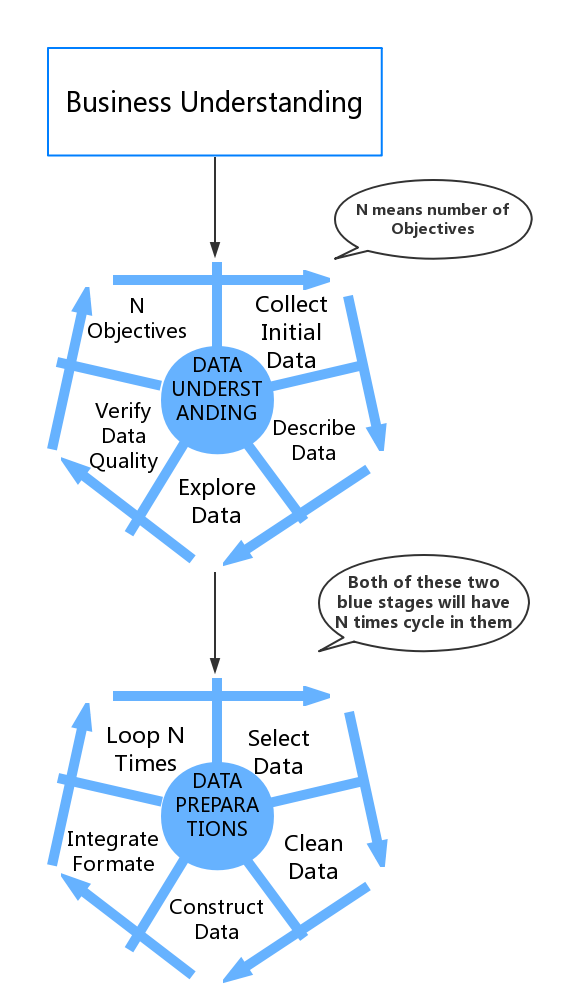
\includegraphics{myloop.png}
\end{itemize}

    \#\#

Start at Business understanding 

    With the development of society and science,data analysing becoming more
and more sophisticated and widely use. This project focus on using
EDA(Exploratory Data Analysis) to find something from Cyber Security
Online Course in Newcastle University by CRISP-DM model. So that the
improvement will make the course, this type of education better in the
future.

Background inOnline Learning Newcastle:

\begin{figure}
\centering
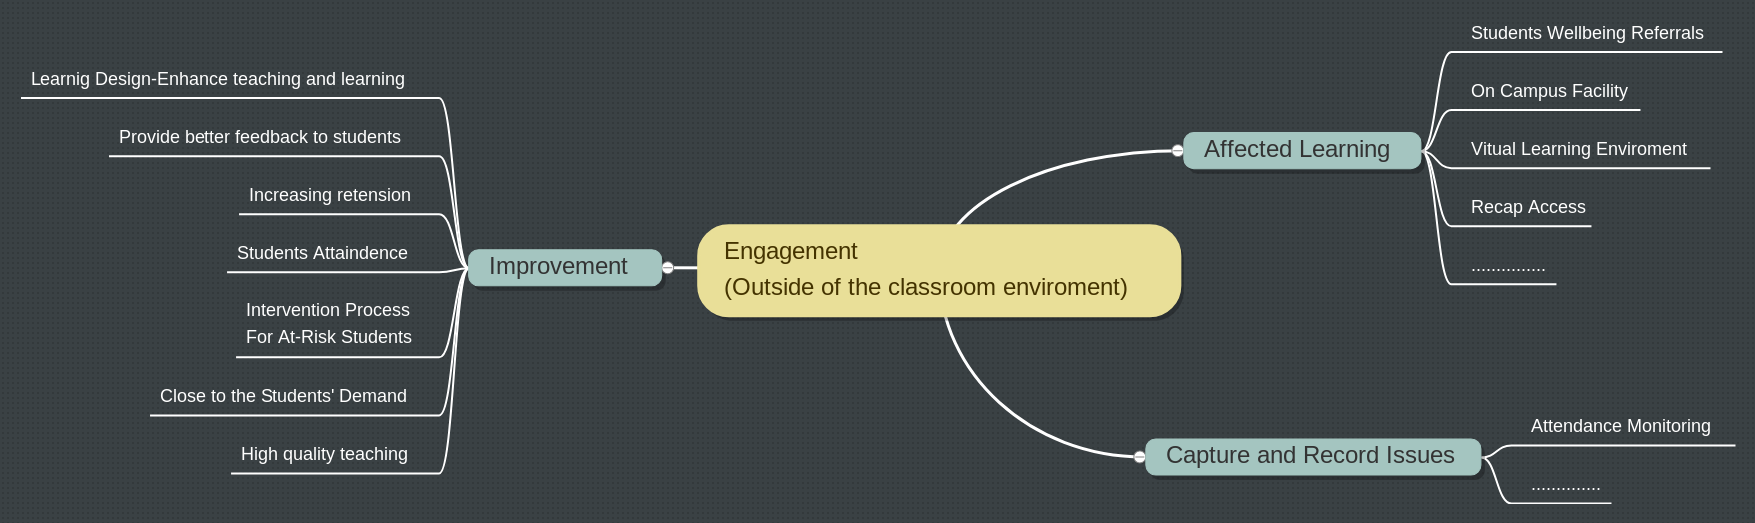
\includegraphics{../reports/figures/bgs.png}
\caption{}
\end{figure}

    \subparagraph{Tools :}\label{tools}

\begin{itemize}
\tightlist
\item
  Ubuntu 16.04 system
\item
  Git and Github for the Version Control
\item
  Cookiecutter for the reproducable ProjectTemplate
\item
  Python for EDA : Numpy, Pandas, Matplotlib, Plotly, Google API
\item
  Jupyter notebook -\/- 'Literate Programming'
\item
  for Sorftware Testing
\end{itemize}

\paragraph{Resource :}\label{resource}

\begin{itemize}
\tightlist
\item
  Newcastle Cyber Security Online learning course Data
\end{itemize}

    Also with the help of Dr Matthew Forshaw who is the is the Technical
Advisor and Dr ... who has rich experinces in education, we can define
the business objective as:

\begin{itemize}
\tightlist
\item
  As a international well konwn university, the course should design
  very well for all the students who comes from whole world, it is
  better for attracting more students whole world.
\item
  The level of difficulty of this course should be balance and
  appropriate for all students in order to keep the completion and help
  students to understand them.
\item
  The custom churn can be interpreted as students churn problem,it is
  very important to know the why students left this course, why they
  can't complete or why they don't want to continue.
\end{itemize}

    \#\#

Data Understanding

    \subsubsection{Our data was collected from a online course in Newcastle
University named : Cyber Security. And the data has the type of `static
data' and `fluid data'. The `static data' is the data collected
traditionally by some institution, they can be the all kinds of records
in university. The `fluid data' is collected from daily activity like
swiping the card, login to the virtual online learning classroom. There
are seven times of this course data we have and was ordered as
cyber-security-1 to cyber-security-7, each of time means a new loop of
this course. And many necessary meaningful data were recorded(We will
check them
later).}\label{our-data-was-collected-from-a-online-course-in-newcastle-university-named-cyber-security.-and-the-data-has-the-type-of-static-data-and-fluid-data.-the-static-data-is-the-data-collected-traditionally-by-some-institution-they-can-be-the-all-kinds-of-records-in-university.-the-fluid-data-is-collected-from-daily-activity-like-swiping-the-card-login-to-the-virtual-online-learning-classroom.-there-are-seven-times-of-this-course-data-we-have-and-was-ordered-as-cyber-security-1-to-cyber-security-7-each-of-time-means-a-new-loop-of-this-course.-and-many-necessary-meaningful-data-were-recordedwe-will-check-them-later.}

    \paragraph{The unusual value will be processed as
:}\label{the-unusual-value-will-be-processed-as}

\begin{longtable}[]{@{}ll@{}}
\toprule
Type & Solution\tabularnewline
\midrule
\endhead
NaN for not used data & Ignore\tabularnewline
Unknown in Enrolment & Ignore and Delete\tabularnewline
Unknown\_2 & shutdown\tabularnewline
Unknown\_3 & shutdown\tabularnewline
\bottomrule
\end{longtable}

\begin{itemize}
\tightlist
\item
  Note: If the unknown value should be replaced, the Unknown continuouse
  values will be replaced by median values of this column because of the
  robust poperty.
\end{itemize}

    \begin{Verbatim}[commandchars=\\\{\}]
{\color{incolor}In [{\color{incolor}231}]:} \PY{c+c1}{\PYZsh{}This is for necessary analysis dependence}
          
          \PY{k+kn}{import} \PY{n+nn}{numpy} \PY{k}{as} \PY{n+nn}{np}
          \PY{k+kn}{from} \PY{n+nn}{geopy}\PY{n+nn}{.}\PY{n+nn}{geocoders} \PY{k}{import} \PY{n}{Nominatim}
          \PY{k+kn}{import} \PY{n+nn}{matplotlib}\PY{n+nn}{.}\PY{n+nn}{pyplot} \PY{k}{as} \PY{n+nn}{plt}
          \PY{k+kn}{import} \PY{n+nn}{plotly} 
          \PY{n}{plotly}\PY{o}{.}\PY{n}{tools}\PY{o}{.}\PY{n}{set\PYZus{}credentials\PYZus{}file}\PY{p}{(}\PY{n}{username}\PY{o}{=}\PY{l+s+s1}{\PYZsq{}}\PY{l+s+s1}{haoran88}\PY{l+s+s1}{\PYZsq{}}\PY{p}{,} \PY{n}{api\PYZus{}key}\PY{o}{=}\PY{l+s+s1}{\PYZsq{}}\PY{l+s+s1}{vrWPoiiR7GpTYytENIAB}\PY{l+s+s1}{\PYZsq{}}\PY{p}{)}
          \PY{k+kn}{import} \PY{n+nn}{pandas} \PY{k}{as} \PY{n+nn}{pd}
          \PY{k+kn}{import} \PY{n+nn}{sklearn}
          \PY{k+kn}{from} \PY{n+nn}{os} \PY{k}{import} \PY{n}{listdir}
          \PY{k+kn}{import} \PY{n+nn}{os}
          \PY{k+kn}{import} \PY{n+nn}{sys}
          \PY{n}{module\PYZus{}path} \PY{o}{=} \PY{n}{os}\PY{o}{.}\PY{n}{path}\PY{o}{.}\PY{n}{abspath}\PY{p}{(}\PY{n}{os}\PY{o}{.}\PY{n}{path}\PY{o}{.}\PY{n}{join}\PY{p}{(}\PY{l+s+s1}{\PYZsq{}}\PY{l+s+s1}{..}\PY{l+s+s1}{\PYZsq{}}\PY{p}{)}\PY{p}{)}
          \PY{k}{if} \PY{n}{module\PYZus{}path} \PY{o+ow}{not} \PY{o+ow}{in} \PY{n}{sys}\PY{o}{.}\PY{n}{path}\PY{p}{:}
              \PY{n}{sys}\PY{o}{.}\PY{n}{path}\PY{o}{.}\PY{n}{append}\PY{p}{(}\PY{n}{module\PYZus{}path}\PY{p}{)}
          \PY{k+kn}{from} \PY{n+nn}{src}\PY{n+nn}{.}\PY{n+nn}{data} \PY{k}{import} \PY{n}{EDA}\PY{p}{,}\PY{n}{Data\PYZus{}Loader}
          \PY{k+kn}{import} \PY{n+nn}{csv}
          \PY{k+kn}{from} \PY{n+nn}{IPython}\PY{n+nn}{.}\PY{n+nn}{display} \PY{k}{import} \PY{n}{display}
          \PY{k+kn}{from} \PY{n+nn}{time} \PY{k}{import} \PY{n}{time}
          
          \PY{o}{\PYZpc{}}\PY{k}{matplotlib} inline
\end{Verbatim}


    data.shape data.info head() tail()
data.info(),data.shape,data.head(),data.tail()

    \begin{Verbatim}[commandchars=\\\{\}]
{\color{incolor}In [{\color{incolor}57}]:} \PY{c+c1}{\PYZsh{}Using the Relative Path is easy to reproduce the project }
         \PY{n}{Main\PYZus{}Data\PYZus{}Path} \PY{o}{=} \PY{l+s+s1}{\PYZsq{}}\PY{l+s+s1}{../Data/raw/Engagement of Cyber Serurity/dataset201819/}\PY{l+s+s1}{\PYZsq{}}
         \PY{n}{data\PYZus{}file\PYZus{}name} \PY{o}{=} \PY{n+nb}{sorted}\PY{p}{(}\PY{n}{listdir}\PY{p}{(}\PY{n}{Main\PYZus{}Data\PYZus{}Path}\PY{p}{)}\PY{p}{)}
\end{Verbatim}


    \begin{Verbatim}[commandchars=\\\{\}]
{\color{incolor}In [{\color{incolor}60}]:} \PY{c+c1}{\PYZsh{}\PYZsh{}\PYZsh{}\PYZsh{} Check all the data we have, check the type of data}
         \PY{n}{num\PYZus{}times} \PY{o}{=} \PY{l+m+mi}{1}
         \PY{n}{times\PYZus{}list} \PY{o}{=} \PY{p}{[}\PY{p}{]}
         \PY{n}{times\PYZus{}count} \PY{o}{=} \PY{p}{[}\PY{p}{]}
         \PY{n}{tmp\PYZus{}data} \PY{o}{=} \PY{p}{[}\PY{p}{]}
         \PY{n}{length\PYZus{}each} \PY{o}{=} \PY{p}{[}\PY{p}{]}
         \PY{n}{nameCount} \PY{o}{=} \PY{p}{[}\PY{p}{]}
         \PY{n}{just\PYZus{}count} \PY{o}{=} \PY{l+m+mi}{0}
         
         \PY{k}{for} \PY{n}{i} \PY{o+ow}{in} \PY{n+nb}{range}\PY{p}{(}\PY{n+nb}{len}\PY{p}{(}\PY{n}{data\PYZus{}file\PYZus{}name}\PY{p}{)} \PY{o}{+} \PY{l+m+mi}{1}\PY{p}{)}\PY{p}{:}
             
             \PY{k}{if} \PY{n}{i} \PY{o}{\PYZgt{}}\PY{o}{=} \PY{n+nb}{len}\PY{p}{(}\PY{n}{data\PYZus{}file\PYZus{}name}\PY{p}{)}\PY{p}{:}
                 \PY{n}{times\PYZus{}list}\PY{o}{.}\PY{n}{append}\PY{p}{(}\PY{n}{tmp\PYZus{}data}\PY{p}{)}
                 \PY{n}{nameCount}\PY{o}{.}\PY{n}{append}\PY{p}{(}\PY{l+s+s1}{\PYZsq{}}\PY{l+s+s1}{Term\PYZus{}}\PY{l+s+s1}{\PYZsq{}}\PY{o}{+}\PY{n+nb}{str}\PY{p}{(}\PY{n}{num\PYZus{}times}\PY{p}{)}\PY{p}{)}
             \PY{k}{else}\PY{p}{:}
                 \PY{k}{if} \PY{n+nb}{int}\PY{p}{(}\PY{n}{data\PYZus{}file\PYZus{}name}\PY{p}{[}\PY{n}{i}\PY{p}{]}\PY{p}{[}\PY{l+m+mi}{15}\PY{p}{]}\PY{p}{)} \PY{o}{!=} \PY{n}{num\PYZus{}times}\PY{p}{:}
                     \PY{n}{length\PYZus{}each}\PY{o}{.}\PY{n}{append}\PY{p}{(}\PY{n}{i} \PY{o}{\PYZhy{}} \PY{n}{just\PYZus{}count}\PY{p}{)}
                     \PY{n}{nameCount}\PY{o}{.}\PY{n}{append}\PY{p}{(}\PY{l+s+s1}{\PYZsq{}}\PY{l+s+s1}{Term\PYZus{}}\PY{l+s+s1}{\PYZsq{}}\PY{o}{+}\PY{n+nb}{str}\PY{p}{(}\PY{n}{num\PYZus{}times}\PY{p}{)}\PY{p}{)}
                     \PY{n}{num\PYZus{}times} \PY{o}{+}\PY{o}{=} \PY{l+m+mi}{1}
                     \PY{n}{times\PYZus{}list}\PY{o}{.}\PY{n}{append}\PY{p}{(}\PY{n}{tmp\PYZus{}data}\PY{p}{)}
                     \PY{n}{tmp\PYZus{}data} \PY{o}{=} \PY{p}{[}\PY{p}{]}
                     \PY{n}{just\PYZus{}count} \PY{o}{=} \PY{n}{i}
                 \PY{c+c1}{\PYZsh{}print(num\PYZus{}times)}
                 \PY{n}{tmp\PYZus{}data}\PY{o}{.}\PY{n}{append}\PY{p}{(}\PY{n}{data\PYZus{}file\PYZus{}name}\PY{p}{[}\PY{n}{i}\PY{p}{]}\PY{p}{[}\PY{l+m+mi}{17}\PY{p}{:}\PY{o}{\PYZhy{}}\PY{l+m+mi}{4}\PY{p}{]}\PY{p}{)}
                 \PY{n}{times\PYZus{}count}\PY{o}{.}\PY{n}{append}\PY{p}{(}\PY{l+s+s1}{\PYZsq{}}\PY{l+s+s1}{Term\PYZus{}}\PY{l+s+s1}{\PYZsq{}}\PY{o}{+}\PY{n+nb}{str}\PY{p}{(}\PY{n}{num\PYZus{}times}\PY{p}{)}\PY{p}{)}
         \PY{n}{data\PYZus{}file} \PY{o}{=} \PY{n}{pd}\PY{o}{.}\PY{n}{DataFrame}\PY{p}{(}\PY{n}{times\PYZus{}list}\PY{p}{,}\PY{n}{index}\PY{o}{=}\PY{n}{nameCount}\PY{p}{)}
         \PY{n+nb}{print}\PY{p}{(}\PY{l+s+s1}{\PYZsq{}}\PY{l+s+s1}{                                                      Fig 1}\PY{l+s+s1}{\PYZsq{}}\PY{p}{)}
         \PY{n}{display}\PY{p}{(}\PY{n}{data\PYZus{}file}\PY{p}{)}
\end{Verbatim}


    \begin{Verbatim}[commandchars=\\\{\}]
                                                      Fig 1

    \end{Verbatim}

    
    \begin{verbatim}
                                 0           1                         2  \
Term_1  archetype-survey-responses  enrolments  leaving-survey-responses   
Term_2  archetype-survey-responses  enrolments  leaving-survey-responses   
Term_3  archetype-survey-responses  enrolments  leaving-survey-responses   
Term_4  archetype-survey-responses  enrolments  leaving-survey-responses   
Term_5  archetype-survey-responses  enrolments  leaving-survey-responses   
Term_6  archetype-survey-responses  enrolments  leaving-survey-responses   
Term_7  archetype-survey-responses  enrolments  leaving-survey-responses   
Term_8                  enrolments        None                      None   

                        3              4                                  5  \
Term_1  question-response  step-activity  weekly-sentiment-survey-responses   
Term_2  question-response  step-activity                       team-members   
Term_3  question-response  step-activity                       team-members   
Term_4  question-response  step-activity                       team-members   
Term_5  question-response  step-activity                       team-members   
Term_6  question-response  step-activity                       team-members   
Term_7  question-response  step-activity                       team-members   
Term_8               None           None                               None   

                                        6                                  7  
Term_1                               None                               None  
Term_2  weekly-sentiment-survey-responses                               None  
Term_3                        video-stats  weekly-sentiment-survey-responses  
Term_4                        video-stats  weekly-sentiment-survey-responses  
Term_5                        video-stats  weekly-sentiment-survey-responses  
Term_6                        video-stats  weekly-sentiment-survey-responses  
Term_7                        video-stats  weekly-sentiment-survey-responses  
Term_8                               None                               None  
    \end{verbatim}

    
    \paragraph{In my opinion, the first and second terms course can't be
used for analyse, because there are many uncertainty and additional
matters in the period of start. Also, as the table shows the first and
second terms lack some informations. So, in this project, we focus on
using the data from terms
3-7.}\label{in-my-opinion-the-first-and-second-terms-course-cant-be-used-for-analyse-because-there-are-many-uncertainty-and-additional-matters-in-the-period-of-start.-also-as-the-table-shows-the-first-and-second-terms-lack-some-informations.-so-in-this-project-we-focus-on-using-the-data-from-terms-3-7.}

\paragraph{All the data were recorded as a '.csv' which is a comma
separated values file which allows data to be saved in a table
structured format. It is convient for us to use tools to load and use
directly without any changes of type of
file.}\label{all-the-data-were-recorded-as-a-.csv-which-is-a-comma-separated-values-file-which-allows-data-to-be-saved-in-a-table-structured-format.-it-is-convient-for-us-to-use-tools-to-load-and-use-directly-without-any-changes-of-type-of-file.}

    \paragraph{For the first Objective, it can be infer that we need to use
the detail of students, so students will give thier personal information
when they first enrolled into this course.So start from the data named
'Cyber-Security-(3-7)\_enrolment.csv' .And then merge all the enrollment
data from term 3 to term 7 ( As big
data)}\label{for-the-first-objective-it-can-be-infer-that-we-need-to-use-the-detail-of-students-so-students-will-give-thier-personal-information-when-they-first-enrolled-into-this-course.so-start-from-the-data-named-cyber-security-3-7_enrolment.csv-.and-then-merge-all-the-enrollment-data-from-term-3-to-term-7-as-big-data}

    \begin{Verbatim}[commandchars=\\\{\}]
{\color{incolor}In [{\color{incolor} }]:} \PY{c+c1}{\PYZsh{}This is our original data}
        \PY{n}{Main\PYZus{}Data\PYZus{}Path} \PY{o}{=} \PY{l+s+s1}{\PYZsq{}}\PY{l+s+s1}{../Data/raw/Engagement of Cyber Serurity/dataset201819/}\PY{l+s+s1}{\PYZsq{}}
        \PY{n}{data\PYZus{}file\PYZus{}name} \PY{o}{=} \PY{n+nb}{sorted}\PY{p}{(}\PY{n}{listdir}\PY{p}{(}\PY{n}{Main\PYZus{}Data\PYZus{}Path}\PY{p}{)}
\end{Verbatim}


    \subsection{Objective 1}\label{objective-1}

    \subsubsection{The point is to attract student, check the Fig 1, the
first thing is to check the basic details and backgrounds of student, so
we check the one enrolments randomly choose term
7.}\label{the-point-is-to-attract-student-check-the-fig-1-the-first-thing-is-to-check-the-basic-details-and-backgrounds-of-student-so-we-check-the-one-enrolments-randomly-choose-term-7.}

    \begin{Verbatim}[commandchars=\\\{\}]
{\color{incolor}In [{\color{incolor}187}]:} \PY{n}{tNum} \PY{o}{=} \PY{l+m+mi}{7}
          \PY{n}{type\PYZus{}file} \PY{o}{=} \PY{l+s+s1}{\PYZsq{}}\PY{l+s+s1}{enrolments}\PY{l+s+s1}{\PYZsq{}}
          \PY{n}{outputPath} \PY{o}{=} \PY{l+s+s1}{\PYZsq{}}\PY{l+s+s1}{../data/processed/}\PY{l+s+s1}{\PYZsq{}} \PY{o}{+} \PY{l+s+s1}{\PYZsq{}}\PY{l+s+s1}{Merged}\PY{l+s+s1}{\PYZsq{}} \PY{o}{+} \PY{n+nb}{str}\PY{p}{(}\PY{n}{startNum}\PY{p}{)} \PY{o}{+} \PY{l+s+s1}{\PYZsq{}}\PY{l+s+s1}{\PYZhy{}}\PY{l+s+s1}{\PYZsq{}} \PY{o}{+} \PY{n+nb}{str}\PY{p}{(}\PY{n}{endNum}\PY{p}{)} \PY{o}{+} \PY{l+s+s1}{\PYZsq{}}\PY{l+s+s1}{\PYZus{}}\PY{l+s+s1}{\PYZsq{}} \PY{o}{+} \PY{n}{type\PYZus{}file} \PY{o}{+} \PY{l+s+s1}{\PYZsq{}}\PY{l+s+s1}{.csv}\PY{l+s+s1}{\PYZsq{}}
          \PY{n}{data\PYZus{}t} \PY{o}{=} \PY{p}{[}\PY{p}{]}
          \PY{n}{timesName} \PY{o}{=} \PY{l+s+s1}{\PYZsq{}}\PY{l+s+s1}{\PYZhy{}}\PY{l+s+s1}{\PYZsq{}} \PY{o}{+} \PY{n+nb}{str}\PY{p}{(}\PY{n}{tNum}\PY{p}{)} \PY{o}{+} \PY{l+s+s1}{\PYZsq{}}\PY{l+s+s1}{\PYZus{}}\PY{l+s+s1}{\PYZsq{}}
          \PY{n}{fileName} \PY{o}{=} \PY{l+s+s1}{\PYZsq{}}\PY{l+s+s1}{../Data/raw/Engagement of Cyber Serurity/dataset201819/cyber\PYZhy{}security}\PY{l+s+s1}{\PYZsq{}} \PY{o}{+} \PY{n}{timesName} \PY{o}{+} \PY{n}{type\PYZus{}file} \PY{o}{+} \PY{l+s+s1}{\PYZsq{}}\PY{l+s+s1}{.csv}\PY{l+s+s1}{\PYZsq{}}
          \PY{n}{data} \PY{o}{=} \PY{n}{pd}\PY{o}{.}\PY{n}{read\PYZus{}csv}\PY{p}{(}\PY{n}{fileName}\PY{p}{)}
          \PY{n}{data\PYZus{}t}\PY{o}{.}\PY{n}{append}\PY{p}{(}\PY{n}{data}\PY{p}{)}
          
          \PY{n}{singlefile} \PY{o}{=} \PY{n}{pd}\PY{o}{.}\PY{n}{read\PYZus{}csv}\PY{p}{(}\PY{n}{fileName}\PY{p}{)}
          \PY{n}{singlefile}\PY{o}{.}\PY{n}{head}\PY{p}{(}\PY{p}{)}
          \PY{c+c1}{\PYZsh{}mergedData.to\PYZus{}csv(outputPath)}
\end{Verbatim}


\begin{Verbatim}[commandchars=\\\{\}]
{\color{outcolor}Out[{\color{outcolor}187}]:}                              learner\_id              enrolled\_at  \textbackslash{}
          0  f0ebc6f6-0f25-407f-a528-834414186f59  2018-10-30 15:14:09 UTC   
          1  0fa1c614-8a49-42a7-a02a-8b866076d552  2018-10-25 12:23:45 UTC   
          2  a0ac585a-eb48-48a8-a34e-b981d9e7b61c  2018-10-23 09:51:07 UTC   
          3  93562e76-6e81-4f8c-8e45-f209d62be693  2018-11-01 11:49:45 UTC   
          4  d1ff90bd-b99b-40c7-a220-ddda5a06bfcd  2018-10-11 11:46:50 UTC   
          
            unenrolled\_at     role fully\_participated\_at purchased\_statement\_at  \textbackslash{}
          0           NaN  learner                   NaN                    NaN   
          1           NaN  learner                   NaN                    NaN   
          2           NaN  learner                   NaN                    NaN   
          3           NaN  learner                   NaN                    NaN   
          4           NaN  learner                   NaN                    NaN   
          
              gender  country age\_range highest\_education\_level employment\_status  \textbackslash{}
          0  Unknown  Unknown   Unknown                 Unknown           Unknown   
          1  Unknown  Unknown   Unknown                 Unknown           Unknown   
          2  Unknown  Unknown   Unknown                 Unknown           Unknown   
          3  Unknown  Unknown   Unknown                 Unknown           Unknown   
          4  Unknown  Unknown   Unknown                 Unknown           Unknown   
          
            employment\_area detected\_country  
          0         Unknown               GB  
          1         Unknown               GB  
          2         Unknown               IN  
          3         Unknown               GB  
          4         Unknown               IQ  
\end{Verbatim}
            
    \begin{Verbatim}[commandchars=\\\{\}]
{\color{incolor}In [{\color{incolor}188}]:} \PY{n}{singlefile} \PY{o}{=} \PY{n}{singlefile}\PY{p}{[}\PY{n}{singlefile}\PY{p}{[}\PY{l+s+s1}{\PYZsq{}}\PY{l+s+s1}{gender}\PY{l+s+s1}{\PYZsq{}}\PY{p}{]} \PY{o}{!=} \PY{l+s+s1}{\PYZsq{}}\PY{l+s+s1}{Unknown}\PY{l+s+s1}{\PYZsq{}}\PY{p}{]}
\end{Verbatim}


    \begin{Verbatim}[commandchars=\\\{\}]
{\color{incolor}In [{\color{incolor}191}]:} \PY{k+kn}{import} \PY{n+nn}{plotly}\PY{n+nn}{.}\PY{n+nn}{plotly} \PY{k}{as} \PY{n+nn}{py}
          \PY{k+kn}{import} \PY{n+nn}{plotly}\PY{n+nn}{.}\PY{n+nn}{graph\PYZus{}objs} \PY{k}{as} \PY{n+nn}{go}
          
          \PY{n+nb}{print}\PY{p}{(}\PY{l+s+s1}{\PYZsq{}}\PY{l+s+s1}{The other genders are just occupy a very little}\PY{l+s+s1}{\PYZsq{}}\PY{p}{)}
          \PY{n+nb}{print}\PY{p}{(}\PY{l+s+s1}{\PYZsq{}}\PY{l+s+s1}{Proportions of the male and female tend to balance.}\PY{l+s+s1}{\PYZsq{}}\PY{p}{)}
          \PY{n+nb}{print}\PY{p}{(}\PY{l+s+s1}{\PYZsq{}}\PY{l+s+s1}{The difference we can asuume that men have more interests in this kind of course}\PY{l+s+s1}{\PYZsq{}}\PY{p}{)}
          
          \PY{n}{labels} \PY{o}{=} \PY{p}{[}\PY{l+s+s1}{\PYZsq{}}\PY{l+s+s1}{Female}\PY{l+s+s1}{\PYZsq{}}\PY{p}{,}\PY{l+s+s1}{\PYZsq{}}\PY{l+s+s1}{Male}\PY{l+s+s1}{\PYZsq{}}\PY{p}{,}\PY{l+s+s1}{\PYZsq{}}\PY{l+s+s1}{Other}\PY{l+s+s1}{\PYZsq{}}\PY{p}{]}
          \PY{n}{values} \PY{o}{=} \PY{p}{[}\PY{n+nb}{float}\PY{p}{(}\PY{n+nb}{len}\PY{p}{(}\PY{n}{singlefile}\PY{p}{[}\PY{n}{singlefile}\PY{p}{[}\PY{l+s+s1}{\PYZsq{}}\PY{l+s+s1}{gender}\PY{l+s+s1}{\PYZsq{}}\PY{p}{]} \PY{o}{==} \PY{l+s+s1}{\PYZsq{}}\PY{l+s+s1}{female}\PY{l+s+s1}{\PYZsq{}}\PY{p}{]}\PY{p}{)}\PY{p}{)} \PY{o}{/} \PY{n+nb}{float}\PY{p}{(}\PY{n+nb}{len}\PY{p}{(}\PY{n}{singlefile}\PY{p}{[}\PY{l+s+s1}{\PYZsq{}}\PY{l+s+s1}{gender}\PY{l+s+s1}{\PYZsq{}}\PY{p}{]}\PY{p}{)}\PY{p}{)} \PY{p}{,}
                    \PY{n+nb}{float}\PY{p}{(}\PY{n+nb}{len}\PY{p}{(}\PY{n}{singlefile}\PY{p}{[}\PY{n}{singlefile}\PY{p}{[}\PY{l+s+s1}{\PYZsq{}}\PY{l+s+s1}{gender}\PY{l+s+s1}{\PYZsq{}}\PY{p}{]} \PY{o}{==} \PY{l+s+s1}{\PYZsq{}}\PY{l+s+s1}{male}\PY{l+s+s1}{\PYZsq{}}\PY{p}{]}\PY{p}{)}\PY{p}{)} \PY{o}{/} \PY{n+nb}{float}\PY{p}{(}\PY{n+nb}{len}\PY{p}{(}\PY{n}{singlefile}\PY{p}{[}\PY{l+s+s1}{\PYZsq{}}\PY{l+s+s1}{gender}\PY{l+s+s1}{\PYZsq{}}\PY{p}{]}\PY{p}{)}\PY{p}{)} \PY{p}{,}
                    \PY{n+nb}{float}\PY{p}{(}\PY{n+nb}{len}\PY{p}{(}\PY{n}{singlefile}\PY{p}{[}\PY{n}{singlefile}\PY{p}{[}\PY{l+s+s1}{\PYZsq{}}\PY{l+s+s1}{gender}\PY{l+s+s1}{\PYZsq{}}\PY{p}{]} \PY{o}{==} \PY{l+s+s1}{\PYZsq{}}\PY{l+s+s1}{other}\PY{l+s+s1}{\PYZsq{}}\PY{p}{]}\PY{p}{)}\PY{p}{)} \PY{o}{/} \PY{n+nb}{float}\PY{p}{(}\PY{n+nb}{len}\PY{p}{(}\PY{n}{singlefile}\PY{p}{[}\PY{l+s+s1}{\PYZsq{}}\PY{l+s+s1}{gender}\PY{l+s+s1}{\PYZsq{}}\PY{p}{]}\PY{p}{)}\PY{p}{)}\PY{p}{]}
          
          \PY{n}{trace} \PY{o}{=} \PY{n}{go}\PY{o}{.}\PY{n}{Pie}\PY{p}{(}\PY{n}{labels}\PY{o}{=}\PY{n}{labels}\PY{p}{,} \PY{n}{values}\PY{o}{=}\PY{n}{values}\PY{p}{)}
          
          \PY{n}{py}\PY{o}{.}\PY{n}{iplot}\PY{p}{(}\PY{p}{[}\PY{n}{trace}\PY{p}{]}\PY{p}{,} \PY{n}{filename}\PY{o}{=}\PY{l+s+s1}{\PYZsq{}}\PY{l+s+s1}{basic\PYZus{}pie\PYZus{}chart}\PY{l+s+s1}{\PYZsq{}}\PY{p}{)}
\end{Verbatim}


    \begin{Verbatim}[commandchars=\\\{\}]
The other genders are just occupy a very little
Proportions of the male and female tend to balance.
The difference we can asuume that men have more interests in this kind of course

    \end{Verbatim}

\begin{Verbatim}[commandchars=\\\{\}]
{\color{outcolor}Out[{\color{outcolor}191}]:} <plotly.tools.PlotlyDisplay object>
\end{Verbatim}
            
    If the number of international students enrolled in this course more
than one third in all the students, it is necessary to make some
additional design for them, such as the subtitles in recap.

    \begin{Verbatim}[commandchars=\\\{\}]
{\color{incolor}In [{\color{incolor}177}]:} \PY{k+kn}{import} \PY{n+nn}{plotly}\PY{n+nn}{.}\PY{n+nn}{plotly} \PY{k}{as} \PY{n+nn}{py}
          \PY{k+kn}{import} \PY{n+nn}{plotly}\PY{n+nn}{.}\PY{n+nn}{graph\PYZus{}objs} \PY{k}{as} \PY{n+nn}{go}
          \PY{n}{singlefile} \PY{o}{=} \PY{n}{singlefile}\PY{p}{[}\PY{n}{singlefile}\PY{p}{[}\PY{l+s+s1}{\PYZsq{}}\PY{l+s+s1}{detected\PYZus{}country}\PY{l+s+s1}{\PYZsq{}}\PY{p}{]} \PY{o}{!=} \PY{l+s+s1}{\PYZsq{}}\PY{l+s+s1}{Unknown}\PY{l+s+s1}{\PYZsq{}}\PY{p}{]}
          \PY{n}{country} \PY{o}{=} \PY{n}{singlefile}\PY{p}{[}\PY{l+s+s1}{\PYZsq{}}\PY{l+s+s1}{detected\PYZus{}country}\PY{l+s+s1}{\PYZsq{}}\PY{p}{]}
          
          \PY{n}{re} \PY{o}{=} \PY{n}{pd}\PY{o}{.}\PY{n}{value\PYZus{}counts}\PY{p}{(}\PY{n}{country}\PY{p}{)}
          
          \PY{n}{re\PYZus{}vale} \PY{o}{=} \PY{n}{re}\PY{o}{.}\PY{n}{tolist}\PY{p}{(}\PY{p}{)}\PY{p}{[}\PY{l+m+mi}{0}\PY{p}{:}\PY{l+m+mi}{20}\PY{p}{]}
          \PY{n}{re\PYZus{}name} \PY{o}{=} \PY{n}{re}\PY{o}{.}\PY{n}{index}\PY{o}{.}\PY{n}{tolist}\PY{p}{(}\PY{p}{)}\PY{p}{[}\PY{l+m+mi}{0}\PY{p}{:}\PY{l+m+mi}{20}\PY{p}{]}
          \PY{n+nb}{print}\PY{p}{(}\PY{l+s+s1}{\PYZsq{}}\PY{l+s+s1}{Chosing tweenty countries(Number of students in other countries are too small to represent) to check the Population }\PY{l+s+s1}{\PYZsq{}}\PY{p}{)}
          
          
          
          \PY{n}{trace0} \PY{o}{=} \PY{n}{go}\PY{o}{.}\PY{n}{Bar}\PY{p}{(}
              \PY{n}{x}\PY{o}{=}\PY{n}{re\PYZus{}name}\PY{p}{,}
              \PY{n}{y}\PY{o}{=}\PY{n}{re\PYZus{}vale}\PY{p}{,}
              \PY{n}{marker}\PY{o}{=}\PY{n+nb}{dict}\PY{p}{(}
                  \PY{n}{color}\PY{o}{=}\PY{l+s+s1}{\PYZsq{}}\PY{l+s+s1}{rgb(158,202,225)}\PY{l+s+s1}{\PYZsq{}}\PY{p}{,}
                  \PY{n}{line}\PY{o}{=}\PY{n+nb}{dict}\PY{p}{(}
                      \PY{n}{color}\PY{o}{=}\PY{l+s+s1}{\PYZsq{}}\PY{l+s+s1}{rgb(8,48,107)}\PY{l+s+s1}{\PYZsq{}}\PY{p}{,}
                      \PY{n}{width}\PY{o}{=}\PY{l+m+mf}{1.5}\PY{p}{,}
                  \PY{p}{)}
              \PY{p}{)}\PY{p}{,}
              \PY{n}{opacity}\PY{o}{=}\PY{l+m+mf}{0.6}
          \PY{p}{)}
          
          \PY{n}{data} \PY{o}{=} \PY{p}{[}\PY{n}{trace0}\PY{p}{]}
          \PY{n}{layout} \PY{o}{=} \PY{n}{go}\PY{o}{.}\PY{n}{Layout}\PY{p}{(}
              \PY{n}{title}\PY{o}{=}\PY{l+s+s1}{\PYZsq{}}\PY{l+s+s1}{Different Countries Students in Term 7}\PY{l+s+s1}{\PYZsq{}}\PY{p}{,}
          \PY{p}{)}
          
          \PY{n}{fig} \PY{o}{=} \PY{n}{go}\PY{o}{.}\PY{n}{Figure}\PY{p}{(}\PY{n}{data}\PY{o}{=}\PY{n}{data}\PY{p}{,} \PY{n}{layout}\PY{o}{=}\PY{n}{layout}\PY{p}{)}
          \PY{n}{py}\PY{o}{.}\PY{n}{iplot}\PY{p}{(}\PY{n}{fig}\PY{p}{,} \PY{n}{filename}\PY{o}{=}\PY{l+s+s1}{\PYZsq{}}\PY{l+s+s1}{text\PYZhy{}hover\PYZhy{}bar}\PY{l+s+s1}{\PYZsq{}}\PY{p}{)}
\end{Verbatim}


    \begin{Verbatim}[commandchars=\\\{\}]
Chosing tweenty countries(Number of students in other countries are too small to represent) to check the Population 

    \end{Verbatim}

\begin{Verbatim}[commandchars=\\\{\}]
{\color{outcolor}Out[{\color{outcolor}177}]:} <plotly.tools.PlotlyDisplay object>
\end{Verbatim}
            
    \begin{Verbatim}[commandchars=\\\{\}]
{\color{incolor}In [{\color{incolor}179}]:} \PY{n}{tNum} \PY{o}{=} \PY{l+m+mi}{7}
          \PY{n}{type\PYZus{}file} \PY{o}{=} \PY{l+s+s1}{\PYZsq{}}\PY{l+s+s1}{enrolments}\PY{l+s+s1}{\PYZsq{}}
          \PY{n}{data\PYZus{}t} \PY{o}{=} \PY{p}{[}\PY{p}{]}
          \PY{n}{timesName} \PY{o}{=} \PY{l+s+s1}{\PYZsq{}}\PY{l+s+s1}{\PYZhy{}}\PY{l+s+s1}{\PYZsq{}} \PY{o}{+} \PY{n+nb}{str}\PY{p}{(}\PY{n}{tNum}\PY{p}{)} \PY{o}{+} \PY{l+s+s1}{\PYZsq{}}\PY{l+s+s1}{\PYZus{}}\PY{l+s+s1}{\PYZsq{}}
          \PY{n}{fileName} \PY{o}{=} \PY{l+s+s1}{\PYZsq{}}\PY{l+s+s1}{../Data/raw/Engagement of Cyber Serurity/dataset201819/cyber\PYZhy{}security}\PY{l+s+s1}{\PYZsq{}} \PY{o}{+} \PY{n}{timesName} \PY{o}{+} \PY{n}{type\PYZus{}file} \PY{o}{+} \PY{l+s+s1}{\PYZsq{}}\PY{l+s+s1}{.csv}\PY{l+s+s1}{\PYZsq{}}
          
          
          \PY{n}{pie1} \PY{o}{=} \PY{n}{pd}\PY{o}{.}\PY{n}{read\PYZus{}csv}\PY{p}{(}\PY{n}{fileName}\PY{p}{)}
          \PY{n}{pie1} \PY{o}{=} \PY{n}{pie1}\PY{p}{[}\PY{n}{pie1}\PY{p}{[}\PY{l+s+s1}{\PYZsq{}}\PY{l+s+s1}{detected\PYZus{}country}\PY{l+s+s1}{\PYZsq{}}\PY{p}{]} \PY{o}{!=} \PY{l+s+s1}{\PYZsq{}}\PY{l+s+s1}{Unknown}\PY{l+s+s1}{\PYZsq{}}\PY{p}{]}
          \PY{n}{pie1} \PY{o}{=} \PY{n}{pie1}\PY{p}{[}\PY{l+s+s1}{\PYZsq{}}\PY{l+s+s1}{detected\PYZus{}country}\PY{l+s+s1}{\PYZsq{}}\PY{p}{]}
          
          \PY{n}{re} \PY{o}{=} \PY{n}{pd}\PY{o}{.}\PY{n}{value\PYZus{}counts}\PY{p}{(}\PY{n}{pie1}\PY{p}{)}
          
          \PY{n}{re\PYZus{}vale1} \PY{o}{=} \PY{n}{re}\PY{o}{.}\PY{n}{tolist}\PY{p}{(}\PY{p}{)}\PY{p}{[}\PY{l+m+mi}{0}\PY{p}{:}\PY{l+m+mi}{20}\PY{p}{]}
          \PY{n}{re\PYZus{}name1} \PY{o}{=} \PY{n}{re}\PY{o}{.}\PY{n}{index}\PY{o}{.}\PY{n}{tolist}\PY{p}{(}\PY{p}{)}\PY{p}{[}\PY{l+m+mi}{0}\PY{p}{:}\PY{l+m+mi}{20}\PY{p}{]}
          \PY{c+c1}{\PYZsh{}mergedData.to\PYZus{}csv(outputPath)}
          
          \PY{n}{tNum} \PY{o}{=} \PY{l+m+mi}{6}
          \PY{n}{type\PYZus{}file} \PY{o}{=} \PY{l+s+s1}{\PYZsq{}}\PY{l+s+s1}{enrolments}\PY{l+s+s1}{\PYZsq{}}
          \PY{n}{data\PYZus{}t} \PY{o}{=} \PY{p}{[}\PY{p}{]}
          \PY{n}{timesName} \PY{o}{=} \PY{l+s+s1}{\PYZsq{}}\PY{l+s+s1}{\PYZhy{}}\PY{l+s+s1}{\PYZsq{}} \PY{o}{+} \PY{n+nb}{str}\PY{p}{(}\PY{n}{tNum}\PY{p}{)} \PY{o}{+} \PY{l+s+s1}{\PYZsq{}}\PY{l+s+s1}{\PYZus{}}\PY{l+s+s1}{\PYZsq{}}
          \PY{n}{fileName} \PY{o}{=} \PY{l+s+s1}{\PYZsq{}}\PY{l+s+s1}{../Data/raw/Engagement of Cyber Serurity/dataset201819/cyber\PYZhy{}security}\PY{l+s+s1}{\PYZsq{}} \PY{o}{+} \PY{n}{timesName} \PY{o}{+} \PY{n}{type\PYZus{}file} \PY{o}{+} \PY{l+s+s1}{\PYZsq{}}\PY{l+s+s1}{.csv}\PY{l+s+s1}{\PYZsq{}}
          
          
          \PY{n}{pie2} \PY{o}{=} \PY{n}{pd}\PY{o}{.}\PY{n}{read\PYZus{}csv}\PY{p}{(}\PY{n}{fileName}\PY{p}{)}
          \PY{n}{pie2} \PY{o}{=} \PY{n}{pie2}\PY{p}{[}\PY{n}{pie2}\PY{p}{[}\PY{l+s+s1}{\PYZsq{}}\PY{l+s+s1}{detected\PYZus{}country}\PY{l+s+s1}{\PYZsq{}}\PY{p}{]} \PY{o}{!=} \PY{l+s+s1}{\PYZsq{}}\PY{l+s+s1}{Unknown}\PY{l+s+s1}{\PYZsq{}}\PY{p}{]}
          \PY{n}{pie2} \PY{o}{=} \PY{n}{pie2}\PY{p}{[}\PY{l+s+s1}{\PYZsq{}}\PY{l+s+s1}{detected\PYZus{}country}\PY{l+s+s1}{\PYZsq{}}\PY{p}{]}
          
          \PY{n}{re} \PY{o}{=} \PY{n}{pd}\PY{o}{.}\PY{n}{value\PYZus{}counts}\PY{p}{(}\PY{n}{pie2}\PY{p}{)}
          
          \PY{n}{re\PYZus{}vale2} \PY{o}{=} \PY{n}{re}\PY{o}{.}\PY{n}{tolist}\PY{p}{(}\PY{p}{)}\PY{p}{[}\PY{l+m+mi}{0}\PY{p}{:}\PY{l+m+mi}{20}\PY{p}{]}
          \PY{n}{re\PYZus{}name2} \PY{o}{=} \PY{n}{re}\PY{o}{.}\PY{n}{index}\PY{o}{.}\PY{n}{tolist}\PY{p}{(}\PY{p}{)}\PY{p}{[}\PY{l+m+mi}{0}\PY{p}{:}\PY{l+m+mi}{20}\PY{p}{]}
\end{Verbatim}


    \begin{Verbatim}[commandchars=\\\{\}]
{\color{incolor}In [{\color{incolor}186}]:} \PY{k+kn}{import} \PY{n+nn}{plotly}\PY{n+nn}{.}\PY{n+nn}{plotly} \PY{k}{as} \PY{n+nn}{py}
          \PY{k+kn}{import} \PY{n+nn}{plotly}\PY{n+nn}{.}\PY{n+nn}{graph\PYZus{}objs} \PY{k}{as} \PY{n+nn}{go}
          
          \PY{n}{fig} \PY{o}{=} \PY{p}{\PYZob{}}
            \PY{l+s+s2}{\PYZdq{}}\PY{l+s+s2}{data}\PY{l+s+s2}{\PYZdq{}}\PY{p}{:} \PY{p}{[}
              \PY{p}{\PYZob{}}
                \PY{l+s+s2}{\PYZdq{}}\PY{l+s+s2}{values}\PY{l+s+s2}{\PYZdq{}}\PY{p}{:} \PY{n}{re\PYZus{}vale1}\PY{p}{,}
                \PY{l+s+s2}{\PYZdq{}}\PY{l+s+s2}{labels}\PY{l+s+s2}{\PYZdq{}}\PY{p}{:} \PY{n}{re\PYZus{}name1}\PY{p}{,}
                \PY{l+s+s2}{\PYZdq{}}\PY{l+s+s2}{domain}\PY{l+s+s2}{\PYZdq{}}\PY{p}{:} \PY{p}{\PYZob{}}\PY{l+s+s2}{\PYZdq{}}\PY{l+s+s2}{x}\PY{l+s+s2}{\PYZdq{}}\PY{p}{:} \PY{p}{[}\PY{l+m+mi}{0}\PY{p}{,} \PY{o}{.}\PY{l+m+mi}{48}\PY{p}{]}\PY{p}{\PYZcb{}}\PY{p}{,}
                \PY{l+s+s2}{\PYZdq{}}\PY{l+s+s2}{name}\PY{l+s+s2}{\PYZdq{}}\PY{p}{:} \PY{l+s+s2}{\PYZdq{}}\PY{l+s+s2}{Term 6}\PY{l+s+s2}{\PYZdq{}}\PY{p}{,}
                \PY{l+s+s2}{\PYZdq{}}\PY{l+s+s2}{hoverinfo}\PY{l+s+s2}{\PYZdq{}}\PY{p}{:}\PY{l+s+s2}{\PYZdq{}}\PY{l+s+s2}{label+percent+name}\PY{l+s+s2}{\PYZdq{}}\PY{p}{,}
                \PY{l+s+s2}{\PYZdq{}}\PY{l+s+s2}{hole}\PY{l+s+s2}{\PYZdq{}}\PY{p}{:} \PY{o}{.}\PY{l+m+mi}{4}\PY{p}{,}
                \PY{l+s+s2}{\PYZdq{}}\PY{l+s+s2}{type}\PY{l+s+s2}{\PYZdq{}}\PY{p}{:} \PY{l+s+s2}{\PYZdq{}}\PY{l+s+s2}{pie}\PY{l+s+s2}{\PYZdq{}}
              \PY{p}{\PYZcb{}}\PY{p}{,}
              \PY{p}{\PYZob{}}
                \PY{l+s+s2}{\PYZdq{}}\PY{l+s+s2}{values}\PY{l+s+s2}{\PYZdq{}}\PY{p}{:} \PY{n}{re\PYZus{}vale2}\PY{p}{,}
                \PY{l+s+s2}{\PYZdq{}}\PY{l+s+s2}{labels}\PY{l+s+s2}{\PYZdq{}}\PY{p}{:} \PY{n}{re\PYZus{}name2}\PY{p}{,}
                \PY{l+s+s2}{\PYZdq{}}\PY{l+s+s2}{textposition}\PY{l+s+s2}{\PYZdq{}}\PY{p}{:}\PY{l+s+s2}{\PYZdq{}}\PY{l+s+s2}{inside}\PY{l+s+s2}{\PYZdq{}}\PY{p}{,}
                \PY{l+s+s2}{\PYZdq{}}\PY{l+s+s2}{domain}\PY{l+s+s2}{\PYZdq{}}\PY{p}{:} \PY{p}{\PYZob{}}\PY{l+s+s2}{\PYZdq{}}\PY{l+s+s2}{x}\PY{l+s+s2}{\PYZdq{}}\PY{p}{:} \PY{p}{[}\PY{o}{.}\PY{l+m+mi}{52}\PY{p}{,} \PY{l+m+mi}{1}\PY{p}{]}\PY{p}{\PYZcb{}}\PY{p}{,}
                \PY{l+s+s2}{\PYZdq{}}\PY{l+s+s2}{name}\PY{l+s+s2}{\PYZdq{}}\PY{p}{:} \PY{l+s+s2}{\PYZdq{}}\PY{l+s+s2}{Term 7}\PY{l+s+s2}{\PYZdq{}}\PY{p}{,}
                \PY{l+s+s2}{\PYZdq{}}\PY{l+s+s2}{hoverinfo}\PY{l+s+s2}{\PYZdq{}}\PY{p}{:}\PY{l+s+s2}{\PYZdq{}}\PY{l+s+s2}{label+percent+name}\PY{l+s+s2}{\PYZdq{}}\PY{p}{,}
                \PY{l+s+s2}{\PYZdq{}}\PY{l+s+s2}{hole}\PY{l+s+s2}{\PYZdq{}}\PY{p}{:} \PY{o}{.}\PY{l+m+mi}{4}\PY{p}{,}
                \PY{l+s+s2}{\PYZdq{}}\PY{l+s+s2}{type}\PY{l+s+s2}{\PYZdq{}}\PY{p}{:} \PY{l+s+s2}{\PYZdq{}}\PY{l+s+s2}{pie}\PY{l+s+s2}{\PYZdq{}}
              \PY{p}{\PYZcb{}}\PY{p}{]}\PY{p}{,}
            \PY{l+s+s2}{\PYZdq{}}\PY{l+s+s2}{layout}\PY{l+s+s2}{\PYZdq{}}\PY{p}{:} \PY{p}{\PYZob{}}
                  \PY{l+s+s2}{\PYZdq{}}\PY{l+s+s2}{title}\PY{l+s+s2}{\PYZdq{}}\PY{p}{:}\PY{l+s+s2}{\PYZdq{}}\PY{l+s+s2}{Percentage of students come from}\PY{l+s+s2}{\PYZdq{}}\PY{p}{,}
                  \PY{l+s+s2}{\PYZdq{}}\PY{l+s+s2}{annotations}\PY{l+s+s2}{\PYZdq{}}\PY{p}{:} \PY{p}{[}
                      \PY{p}{\PYZob{}}
                          \PY{l+s+s2}{\PYZdq{}}\PY{l+s+s2}{font}\PY{l+s+s2}{\PYZdq{}}\PY{p}{:} \PY{p}{\PYZob{}}
                              \PY{l+s+s2}{\PYZdq{}}\PY{l+s+s2}{size}\PY{l+s+s2}{\PYZdq{}}\PY{p}{:} \PY{l+m+mi}{20}
                          \PY{p}{\PYZcb{}}\PY{p}{,}
                          \PY{l+s+s2}{\PYZdq{}}\PY{l+s+s2}{showarrow}\PY{l+s+s2}{\PYZdq{}}\PY{p}{:} \PY{k+kc}{False}\PY{p}{,}
                          \PY{l+s+s2}{\PYZdq{}}\PY{l+s+s2}{text}\PY{l+s+s2}{\PYZdq{}}\PY{p}{:} \PY{l+s+s2}{\PYZdq{}}\PY{l+s+s2}{Term 6}\PY{l+s+s2}{\PYZdq{}}\PY{p}{,}
                          \PY{l+s+s2}{\PYZdq{}}\PY{l+s+s2}{x}\PY{l+s+s2}{\PYZdq{}}\PY{p}{:} \PY{l+m+mf}{0.20}\PY{p}{,}
                          \PY{l+s+s2}{\PYZdq{}}\PY{l+s+s2}{y}\PY{l+s+s2}{\PYZdq{}}\PY{p}{:} \PY{l+m+mf}{0.5}
                      \PY{p}{\PYZcb{}}\PY{p}{,}
                      \PY{p}{\PYZob{}}
                          \PY{l+s+s2}{\PYZdq{}}\PY{l+s+s2}{font}\PY{l+s+s2}{\PYZdq{}}\PY{p}{:} \PY{p}{\PYZob{}}
                              \PY{l+s+s2}{\PYZdq{}}\PY{l+s+s2}{size}\PY{l+s+s2}{\PYZdq{}}\PY{p}{:} \PY{l+m+mi}{20}
                          \PY{p}{\PYZcb{}}\PY{p}{,}
                          \PY{l+s+s2}{\PYZdq{}}\PY{l+s+s2}{showarrow}\PY{l+s+s2}{\PYZdq{}}\PY{p}{:} \PY{k+kc}{False}\PY{p}{,}
                          \PY{l+s+s2}{\PYZdq{}}\PY{l+s+s2}{text}\PY{l+s+s2}{\PYZdq{}}\PY{p}{:} \PY{l+s+s2}{\PYZdq{}}\PY{l+s+s2}{Term 7}\PY{l+s+s2}{\PYZdq{}}\PY{p}{,}
                          \PY{l+s+s2}{\PYZdq{}}\PY{l+s+s2}{x}\PY{l+s+s2}{\PYZdq{}}\PY{p}{:} \PY{l+m+mf}{0.8}\PY{p}{,}
                          \PY{l+s+s2}{\PYZdq{}}\PY{l+s+s2}{y}\PY{l+s+s2}{\PYZdq{}}\PY{p}{:} \PY{l+m+mf}{0.5}
                      \PY{p}{\PYZcb{}}
                  \PY{p}{]}
              \PY{p}{\PYZcb{}}
          \PY{p}{\PYZcb{}}
          \PY{n}{py}\PY{o}{.}\PY{n}{iplot}\PY{p}{(}\PY{n}{fig}\PY{p}{,} \PY{n}{filename}\PY{o}{=}\PY{l+s+s1}{\PYZsq{}}\PY{l+s+s1}{donut}\PY{l+s+s1}{\PYZsq{}}\PY{p}{)}
\end{Verbatim}


\begin{Verbatim}[commandchars=\\\{\}]
{\color{outcolor}Out[{\color{outcolor}186}]:} <plotly.tools.PlotlyDisplay object>
\end{Verbatim}
            
    \paragraph{It is worth to use the location data to check where students
come from,and design different type of teaching type. What kinds of the
recap should be designed. So for the objective 1, we can use the
enrollments data to analysis with later
work:}\label{it-is-worth-to-use-the-location-data-to-check-where-students-come-fromand-design-different-type-of-teaching-type.-what-kinds-of-the-recap-should-be-designed.-so-for-the-objective-1-we-can-use-the-enrollments-data-to-analysis-with-later-work}

\begin{itemize}
\tightlist
\item
  Merge enrollment data in term3 to term7
\item
  clean and process the unusual data
\end{itemize}

    \subsection{Objective 2}\label{objective-2}

    For the objective of the level of difficulty, coursework is the one of
the most important method to response, check what the proportion of
students who can correctly answer the questions in or out of the online
lecture. If more than half of students can't make it, the level of the
course or some parts of course are inappropriate for many of students.

    \paragraph{Chek the Table 1, there are some files named 'question
response',randomly chooose the term
6:}\label{chek-the-table-1-there-are-some-files-named-question-responserandomly-chooose-the-term-6}

    \begin{Verbatim}[commandchars=\\\{\}]
{\color{incolor}In [{\color{incolor}147}]:} \PY{n}{tNum} \PY{o}{=} \PY{l+m+mi}{6}
          \PY{n}{type\PYZus{}file} \PY{o}{=} \PY{l+s+s1}{\PYZsq{}}\PY{l+s+s1}{question\PYZhy{}response}\PY{l+s+s1}{\PYZsq{}}
          \PY{c+c1}{\PYZsh{}outputPath = \PYZsq{}../data/processed/\PYZsq{} + \PYZsq{}Merged\PYZsq{} + str(startNum) + \PYZsq{}\PYZhy{}\PYZsq{} + str(endNum) + \PYZsq{}\PYZus{}\PYZsq{} + type\PYZus{}file + \PYZsq{}.csv\PYZsq{}}
          \PY{n}{data\PYZus{}t} \PY{o}{=} \PY{p}{[}\PY{p}{]}
          \PY{n}{timesName} \PY{o}{=} \PY{l+s+s1}{\PYZsq{}}\PY{l+s+s1}{\PYZhy{}}\PY{l+s+s1}{\PYZsq{}} \PY{o}{+} \PY{n+nb}{str}\PY{p}{(}\PY{n}{tNum}\PY{p}{)} \PY{o}{+} \PY{l+s+s1}{\PYZsq{}}\PY{l+s+s1}{\PYZus{}}\PY{l+s+s1}{\PYZsq{}}
          \PY{n}{fileName} \PY{o}{=} \PY{l+s+s1}{\PYZsq{}}\PY{l+s+s1}{../Data/raw/Engagement of Cyber Serurity/dataset201819/cyber\PYZhy{}security}\PY{l+s+s1}{\PYZsq{}} \PY{o}{+} \PY{n}{timesName} \PY{o}{+} \PY{n}{type\PYZus{}file} \PY{o}{+} \PY{l+s+s1}{\PYZsq{}}\PY{l+s+s1}{.csv}\PY{l+s+s1}{\PYZsq{}}
          \PY{n}{data} \PY{o}{=} \PY{n}{pd}\PY{o}{.}\PY{n}{read\PYZus{}csv}\PY{p}{(}\PY{n}{fileName}\PY{p}{)}
          \PY{n}{data\PYZus{}t}\PY{o}{.}\PY{n}{append}\PY{p}{(}\PY{n}{data}\PY{p}{)}
          
          \PY{n}{singlefile} \PY{o}{=} \PY{n}{pd}\PY{o}{.}\PY{n}{read\PYZus{}csv}\PY{p}{(}\PY{n}{fileName}\PY{p}{)}
          \PY{n}{singlefile}\PY{o}{.}\PY{n}{head}\PY{p}{(}\PY{p}{)}
          \PY{c+c1}{\PYZsh{}mergedData.to\PYZus{}csv(outputPath)}
\end{Verbatim}


\begin{Verbatim}[commandchars=\\\{\}]
{\color{outcolor}Out[{\color{outcolor}147}]:}                              learner\_id quiz\_question   question\_type  \textbackslash{}
          0  3f5389d8-4b4d-43af-904e-cc32946a4845         1.8.1  MultipleChoice   
          1  6ffbff85-fe97-4fee-994d-17a32bdf867c         1.8.1  MultipleChoice   
          2  b89dd8da-585e-4b2c-953b-c6d475e07099         1.8.1  MultipleChoice   
          3  b89dd8da-585e-4b2c-953b-c6d475e07099         1.8.1  MultipleChoice   
          4  b89dd8da-585e-4b2c-953b-c6d475e07099         1.8.1  MultipleChoice   
          
             week\_number  step\_number  question\_number response  cloze\_response  \textbackslash{}
          0            1            8                1    1,2,3             NaN   
          1            1            8                1    1,2,3             NaN   
          2            1            8                1        3             NaN   
          3            1            8                1      2,3             NaN   
          4            1            8                1    1,2,3             NaN   
          
                        submitted\_at  correct  
          0  2018-06-11 01:18:29 UTC     True  
          1  2018-06-11 01:47:45 UTC     True  
          2  2018-06-11 03:17:42 UTC    False  
          3  2018-06-11 03:17:45 UTC    False  
          4  2018-06-11 03:17:47 UTC     True  
\end{Verbatim}
            
    \paragraph{There is a column named 'correct ',it can show if students
can answer the questions, so that if the performance is good, it can be
assumed that the difficulty of the course is appropriate,but if the
number of worng answer is obviousely big in any question, for example
almost more than half students failed to answer, the director should
consider the level of difficulty or the if the teacher presented a
appropriate
lectures.}\label{there-is-a-column-named-correct-it-can-show-if-students-can-answer-the-questions-so-that-if-the-performance-is-good-it-can-be-assumed-that-the-difficulty-of-the-course-is-appropriatebut-if-the-number-of-worng-answer-is-obviousely-big-in-any-question-for-example-almost-more-than-half-students-failed-to-answer-the-director-should-consider-the-level-of-difficulty-or-the-if-the-teacher-presented-a-appropriate-lectures.}

    \begin{Verbatim}[commandchars=\\\{\}]
{\color{incolor}In [{\color{incolor}161}]:} \PY{n+nb}{print}\PY{p}{(}\PY{n+nb}{type}\PY{p}{(}\PY{n}{singlefile}\PY{p}{[}\PY{l+s+s1}{\PYZsq{}}\PY{l+s+s1}{correct}\PY{l+s+s1}{\PYZsq{}}\PY{p}{]}\PY{p}{[}\PY{l+m+mi}{1}\PY{p}{]}\PY{p}{)}\PY{p}{)}
          \PY{n}{numF} \PY{o}{=} \PY{n+nb}{len}\PY{p}{(}\PY{n}{singlefile}\PY{p}{[}\PY{n}{singlefile}\PY{p}{[}\PY{l+s+s1}{\PYZsq{}}\PY{l+s+s1}{correct}\PY{l+s+s1}{\PYZsq{}}\PY{p}{]} \PY{o}{==} \PY{k+kc}{False}\PY{p}{]}\PY{p}{)}
          \PY{n}{numT} \PY{o}{=} \PY{n+nb}{len}\PY{p}{(}\PY{n}{singlefile}\PY{p}{[}\PY{n}{singlefile}\PY{p}{[}\PY{l+s+s1}{\PYZsq{}}\PY{l+s+s1}{correct}\PY{l+s+s1}{\PYZsq{}}\PY{p}{]} \PY{o}{==} \PY{k+kc}{True}\PY{p}{]}\PY{p}{)}
          
          \PY{n+nb}{print}\PY{p}{(}\PY{n}{numF}\PY{p}{)}
          \PY{n+nb}{print}\PY{p}{(}\PY{n}{numT}\PY{p}{)}
          \PY{n+nb}{print}\PY{p}{(}\PY{n+nb}{len}\PY{p}{(}\PY{n}{pd}\PY{o}{.}\PY{n}{unique}\PY{p}{(}\PY{n}{singlefile}\PY{p}{[}\PY{l+s+s1}{\PYZsq{}}\PY{l+s+s1}{quiz\PYZus{}question}\PY{l+s+s1}{\PYZsq{}}\PY{p}{]}\PY{p}{)}\PY{p}{)}\PY{p}{)}
          
          \PY{n}{question} \PY{o}{=} \PY{n}{pd}\PY{o}{.}\PY{n}{unique}\PY{p}{(}\PY{n}{singlefile}\PY{p}{[}\PY{l+s+s1}{\PYZsq{}}\PY{l+s+s1}{quiz\PYZus{}question}\PY{l+s+s1}{\PYZsq{}}\PY{p}{]}\PY{p}{)}
          
          \PY{n+nb}{print}\PY{p}{(}\PY{n}{question}\PY{p}{)}
          
          \PY{n}{WrongAnswer} \PY{o}{=} \PY{p}{[}\PY{p}{]}
          
          \PY{n}{choose\PYZus{}tmp} \PY{o}{=} \PY{n}{singlefile}\PY{p}{[}\PY{n}{singlefile}\PY{p}{[}\PY{l+s+s1}{\PYZsq{}}\PY{l+s+s1}{correct}\PY{l+s+s1}{\PYZsq{}}\PY{p}{]} \PY{o}{==} \PY{k+kc}{False}\PY{p}{]}
          
          \PY{k}{for} \PY{n}{i} \PY{o+ow}{in} \PY{n}{question}\PY{p}{:}
              \PY{n}{WrongAnswer}\PY{o}{.}\PY{n}{append}\PY{p}{(}\PY{n+nb}{len}\PY{p}{(}\PY{n}{choose\PYZus{}tmp}\PY{p}{[}\PY{n}{choose\PYZus{}tmp}\PY{p}{[}\PY{l+s+s1}{\PYZsq{}}\PY{l+s+s1}{quiz\PYZus{}question}\PY{l+s+s1}{\PYZsq{}}\PY{p}{]} \PY{o}{==} \PY{n}{i}\PY{p}{]}\PY{p}{)}\PY{p}{)}
              
          \PY{n+nb}{print}\PY{p}{(}\PY{n}{WrongAnswer}\PY{p}{)}
\end{Verbatim}


    \begin{Verbatim}[commandchars=\\\{\}]
<class 'numpy.bool\_'>
4486
6047
22
['1.8.1' '1.8.2' '1.8.3' '1.8.4' '1.8.5' '1.8.6' '2.8.1' '2.8.2' '2.8.3'
 '2.20.1' '3.11.1' '3.11.2' '3.11.3' '3.18.1' '3.18.2' '3.18.3' '3.18.4'
 '3.18.5' '3.18.6' '3.18.7' '3.18.8' '3.18.9']
[528, 313, 560, 74, 0, 658, 374, 269, 343, 90, 377, 188, 506, 44, 1, 29, 7, 19, 24, 15, 21, 46]

    \end{Verbatim}

    \begin{Verbatim}[commandchars=\\\{\}]
{\color{incolor}In [{\color{incolor}167}]:} \PY{k+kn}{import} \PY{n+nn}{plotly}\PY{n+nn}{.}\PY{n+nn}{plotly} \PY{k}{as} \PY{n+nn}{py}
          \PY{k+kn}{import} \PY{n+nn}{plotly}\PY{n+nn}{.}\PY{n+nn}{graph\PYZus{}objs} \PY{k}{as} \PY{n+nn}{go}
          
          
          \PY{c+c1}{\PYZsh{} Create traces}
          \PY{n}{trace0} \PY{o}{=} \PY{n}{go}\PY{o}{.}\PY{n}{Scatter}\PY{p}{(}
              \PY{n}{x} \PY{o}{=} \PY{n}{question}\PY{p}{,}
              \PY{n}{y} \PY{o}{=} \PY{n}{WrongAnswer}\PY{p}{,}
              \PY{n}{mode} \PY{o}{=} \PY{l+s+s1}{\PYZsq{}}\PY{l+s+s1}{lines+markers}\PY{l+s+s1}{\PYZsq{}}\PY{p}{,}
              \PY{n}{name} \PY{o}{=} \PY{l+s+s1}{\PYZsq{}}\PY{l+s+s1}{lines+markers}\PY{l+s+s1}{\PYZsq{}}
          \PY{p}{)}
          \PY{n}{data} \PY{o}{=} \PY{p}{[}\PY{n}{trace0}\PY{p}{]}
          
          \PY{n}{py}\PY{o}{.}\PY{n}{iplot}\PY{p}{(}\PY{n}{data}\PY{p}{,} \PY{n}{filename}\PY{o}{=}\PY{l+s+s1}{\PYZsq{}}\PY{l+s+s1}{line\PYZhy{}mode}\PY{l+s+s1}{\PYZsq{}}\PY{p}{)}
\end{Verbatim}


\begin{Verbatim}[commandchars=\\\{\}]
{\color{outcolor}Out[{\color{outcolor}167}]:} <plotly.tools.PlotlyDisplay object>
\end{Verbatim}
            
    \subsection{Objective 3}\label{objective-3}

    The 'csv' data file named leaving-survey-responses recorded the time and
reason that students left.It is very useful if more than one third
students left because of the same reason,or if a reason that has a big
proportion,so the director of this course should focus on improving it.

    \begin{Verbatim}[commandchars=\\\{\}]
{\color{incolor}In [{\color{incolor}192}]:} \PY{n}{tNum} \PY{o}{=} \PY{l+m+mi}{6}
          \PY{n}{type\PYZus{}file} \PY{o}{=} \PY{l+s+s1}{\PYZsq{}}\PY{l+s+s1}{leaving\PYZhy{}survey\PYZhy{}responses}\PY{l+s+s1}{\PYZsq{}}
          \PY{c+c1}{\PYZsh{}outputPath = \PYZsq{}../data/processed/\PYZsq{} + \PYZsq{}Merged\PYZsq{} + str(startNum) + \PYZsq{}\PYZhy{}\PYZsq{} + str(endNum) + \PYZsq{}\PYZus{}\PYZsq{} + type\PYZus{}file + \PYZsq{}.csv\PYZsq{}}
          \PY{n}{data\PYZus{}t} \PY{o}{=} \PY{p}{[}\PY{p}{]}
          \PY{n}{timesName} \PY{o}{=} \PY{l+s+s1}{\PYZsq{}}\PY{l+s+s1}{\PYZhy{}}\PY{l+s+s1}{\PYZsq{}} \PY{o}{+} \PY{n+nb}{str}\PY{p}{(}\PY{n}{tNum}\PY{p}{)} \PY{o}{+} \PY{l+s+s1}{\PYZsq{}}\PY{l+s+s1}{\PYZus{}}\PY{l+s+s1}{\PYZsq{}}
          \PY{n}{fileName} \PY{o}{=} \PY{l+s+s1}{\PYZsq{}}\PY{l+s+s1}{../Data/raw/Engagement of Cyber Serurity/dataset201819/cyber\PYZhy{}security}\PY{l+s+s1}{\PYZsq{}} \PY{o}{+} \PY{n}{timesName} \PY{o}{+} \PY{n}{type\PYZus{}file} \PY{o}{+} \PY{l+s+s1}{\PYZsq{}}\PY{l+s+s1}{.csv}\PY{l+s+s1}{\PYZsq{}}
          
          
          \PY{n}{singlefile} \PY{o}{=} \PY{n}{pd}\PY{o}{.}\PY{n}{read\PYZus{}csv}\PY{p}{(}\PY{n}{fileName}\PY{p}{)}
          \PY{n}{singlefile}\PY{o}{.}\PY{n}{head}\PY{p}{(}\PY{p}{)}
          \PY{c+c1}{\PYZsh{}mergedData.to\PYZus{}csv(outputPath)}
\end{Verbatim}


\begin{Verbatim}[commandchars=\\\{\}]
{\color{outcolor}Out[{\color{outcolor}192}]:}        id                            learner\_id                  left\_at  \textbackslash{}
          0  110338  9f172f7a-74fa-4e6a-991a-cad1aedbce41  2018-04-20 12:12:05 UTC   
          1  120486  353eaf1b-cff8-4d9c-98d4-b9a736c17e73  2018-05-09 03:54:35 UTC   
          2  125315  8c4eee40-70ae-45ef-ab61-cdf2832328b1  2018-05-18 09:10:38 UTC   
          3  126064  c1c34f22-2e36-4fb5-9295-3a92f5f94350  2018-05-20 12:15:19 UTC   
          4  126988  798f378b-858d-44ac-a254-0846625dc7e9  2018-05-21 17:54:05 UTC   
          
                                            leaving\_reason   last\_completed\_step\_at  \textbackslash{}
          0                                          Other                      NaN   
          1  The course required more time than I realised  2018-07-15 16:53:37 UTC   
          2                       I don’t have enough time                      NaN   
          3                            I prefer not to say                      NaN   
          4                                          Other                      NaN   
          
             last\_completed\_step  last\_completed\_week\_number  last\_completed\_step\_number  
          0                  NaN                         NaN                         NaN  
          1                  3.2                         3.0                        20.0  
          2                  NaN                         NaN                         NaN  
          3                  NaN                         NaN                         NaN  
          4                  NaN                         NaN                         NaN  
\end{Verbatim}
            
    \paragraph{I think the director will be interested in why the students
want to leave the course, it is the very important feedback from student
to improve the course in the future.Then we check the column named
'leaving-reason'
:}\label{i-think-the-director-will-be-interested-in-why-the-students-want-to-leave-the-course-it-is-the-very-important-feedback-from-student-to-improve-the-course-in-the-future.then-we-check-the-column-named-leaving-reason}

    \begin{Verbatim}[commandchars=\\\{\}]
{\color{incolor}In [{\color{incolor}249}]:} \PY{n}{a} \PY{o}{=} \PY{n+nb}{dict}\PY{p}{(}\PY{n+nb}{zip}\PY{p}{(}\PY{n}{reasons}\PY{p}{,}\PY{n}{re\PYZus{}va}\PY{p}{)}\PY{p}{)}
          
          \PY{n}{b} \PY{o}{=} \PY{n+nb}{list}\PY{p}{(}\PY{n+nb}{range}\PY{p}{(}\PY{n+nb}{int}\PY{p}{(}\PY{p}{(}\PY{l+m+mi}{1}\PY{o}{/}\PY{l+m+mi}{5}\PY{p}{)} \PY{o}{*} \PY{n+nb}{max}\PY{p}{(}\PY{n}{re\PYZus{}va}\PY{p}{)}\PY{p}{)}\PY{p}{)}\PY{p}{)}
          
          \PY{k}{for} \PY{n}{i} \PY{o+ow}{in} \PY{n}{reasons}\PY{p}{:}
              \PY{k}{if} \PY{n}{a}\PY{p}{[}\PY{n}{i}\PY{p}{]} \PY{o+ow}{in} \PY{n}{b}\PY{p}{:}
                  \PY{n}{a}\PY{o}{.}\PY{n}{pop}\PY{p}{(}\PY{n}{i}\PY{p}{)}
                  
          \PY{n}{reasons} \PY{o}{=} \PY{n+nb}{list}\PY{p}{(}\PY{n}{a}\PY{o}{.}\PY{n}{keys}\PY{p}{(}\PY{p}{)}\PY{p}{)}
          \PY{n}{re\PYZus{}va} \PY{o}{=} \PY{n+nb}{list}\PY{p}{(}\PY{n}{a}\PY{o}{.}\PY{n}{values}\PY{p}{(}\PY{p}{)}\PY{p}{)}
\end{Verbatim}


    \begin{Verbatim}[commandchars=\\\{\}]
{\color{incolor}In [{\color{incolor}250}]:} \PY{c+c1}{\PYZsh{}reasons = pd.unique(singlefile[\PYZsq{}leaving\PYZus{}reason\PYZsq{}])}
          
          \PY{c+c1}{\PYZsh{}reasons = reasons.tolist()}
          \PY{c+c1}{\PYZsh{}re\PYZus{}va = []}
          
          \PY{c+c1}{\PYZsh{}for i in reasons:}
          \PY{c+c1}{\PYZsh{}    re\PYZus{}va.append(len(singlefile[singlefile[\PYZsq{}leaving\PYZus{}reason\PYZsq{}] == i]))}
              
          \PY{c+c1}{\PYZsh{}print(re\PYZus{}va)}
          \PY{c+c1}{\PYZsh{}print(reasons)}
          
          \PY{k+kn}{import} \PY{n+nn}{plotly}\PY{n+nn}{.}\PY{n+nn}{plotly} \PY{k}{as} \PY{n+nn}{py}
          \PY{k+kn}{import} \PY{n+nn}{plotly}\PY{n+nn}{.}\PY{n+nn}{graph\PYZus{}objs} \PY{k}{as} \PY{n+nn}{go}
          
          \PY{k+kn}{import} \PY{n+nn}{squarify}
          
          \PY{n}{x} \PY{o}{=} \PY{l+m+mf}{0.}
          \PY{n}{y} \PY{o}{=} \PY{l+m+mf}{0.}
          \PY{n}{width} \PY{o}{=} \PY{l+m+mf}{100.}
          \PY{n}{height} \PY{o}{=} \PY{l+m+mf}{100.}
          
          \PY{n}{values} \PY{o}{=} \PY{n}{re\PYZus{}va}
          
          \PY{n}{normed} \PY{o}{=} \PY{n}{squarify}\PY{o}{.}\PY{n}{normalize\PYZus{}sizes}\PY{p}{(}\PY{n}{values}\PY{p}{,} \PY{n}{width}\PY{p}{,} \PY{n}{height}\PY{p}{)}
          \PY{n}{rects} \PY{o}{=} \PY{n}{squarify}\PY{o}{.}\PY{n}{squarify}\PY{p}{(}\PY{n}{normed}\PY{p}{,} \PY{n}{x}\PY{p}{,} \PY{n}{y}\PY{p}{,} \PY{n}{width}\PY{p}{,} \PY{n}{height}\PY{p}{)}
          
          \PY{c+c1}{\PYZsh{} Choose colors from http://colorbrewer2.org/ under \PYZdq{}Export\PYZdq{}}
          \PY{n}{color\PYZus{}brewer} \PY{o}{=} \PY{p}{[}\PY{l+s+s1}{\PYZsq{}}\PY{l+s+s1}{rgb(166,206,227)}\PY{l+s+s1}{\PYZsq{}}\PY{p}{,}\PY{l+s+s1}{\PYZsq{}}\PY{l+s+s1}{rgb(31,120,180)}\PY{l+s+s1}{\PYZsq{}}\PY{p}{,}\PY{l+s+s1}{\PYZsq{}}\PY{l+s+s1}{rgb(178,223,138)}\PY{l+s+s1}{\PYZsq{}}\PY{p}{,}
                          \PY{l+s+s1}{\PYZsq{}}\PY{l+s+s1}{rgb(51,160,44)}\PY{l+s+s1}{\PYZsq{}}\PY{p}{,}\PY{l+s+s1}{\PYZsq{}}\PY{l+s+s1}{rgb(251,154,153)}\PY{l+s+s1}{\PYZsq{}}\PY{p}{,}\PY{l+s+s1}{\PYZsq{}}\PY{l+s+s1}{rgb(227,26,28)}\PY{l+s+s1}{\PYZsq{}}\PY{p}{]}
          \PY{n}{shapes} \PY{o}{=} \PY{p}{[}\PY{p}{]}
          \PY{n}{annotations} \PY{o}{=} \PY{p}{[}\PY{p}{]}
          \PY{n}{counter} \PY{o}{=} \PY{l+m+mi}{0}
          
          \PY{k}{for} \PY{n}{r} \PY{o+ow}{in} \PY{n}{rects}\PY{p}{:}
              \PY{n}{shapes}\PY{o}{.}\PY{n}{append}\PY{p}{(} 
                  \PY{n+nb}{dict}\PY{p}{(}
                      \PY{n+nb}{type} \PY{o}{=} \PY{l+s+s1}{\PYZsq{}}\PY{l+s+s1}{rect}\PY{l+s+s1}{\PYZsq{}}\PY{p}{,} 
                      \PY{n}{x0} \PY{o}{=} \PY{n}{r}\PY{p}{[}\PY{l+s+s1}{\PYZsq{}}\PY{l+s+s1}{x}\PY{l+s+s1}{\PYZsq{}}\PY{p}{]}\PY{p}{,} 
                      \PY{n}{y0} \PY{o}{=} \PY{n}{r}\PY{p}{[}\PY{l+s+s1}{\PYZsq{}}\PY{l+s+s1}{y}\PY{l+s+s1}{\PYZsq{}}\PY{p}{]}\PY{p}{,} 
                      \PY{n}{x1} \PY{o}{=} \PY{n}{r}\PY{p}{[}\PY{l+s+s1}{\PYZsq{}}\PY{l+s+s1}{x}\PY{l+s+s1}{\PYZsq{}}\PY{p}{]}\PY{o}{+}\PY{n}{r}\PY{p}{[}\PY{l+s+s1}{\PYZsq{}}\PY{l+s+s1}{dx}\PY{l+s+s1}{\PYZsq{}}\PY{p}{]}\PY{p}{,} 
                      \PY{n}{y1} \PY{o}{=} \PY{n}{r}\PY{p}{[}\PY{l+s+s1}{\PYZsq{}}\PY{l+s+s1}{y}\PY{l+s+s1}{\PYZsq{}}\PY{p}{]}\PY{o}{+}\PY{n}{r}\PY{p}{[}\PY{l+s+s1}{\PYZsq{}}\PY{l+s+s1}{dy}\PY{l+s+s1}{\PYZsq{}}\PY{p}{]}\PY{p}{,}
                      \PY{n}{line} \PY{o}{=} \PY{n+nb}{dict}\PY{p}{(} \PY{n}{width} \PY{o}{=} \PY{l+m+mi}{2} \PY{p}{)}\PY{p}{,}
                      \PY{n}{fillcolor} \PY{o}{=} \PY{n}{color\PYZus{}brewer}\PY{p}{[}\PY{n}{counter}\PY{p}{]}
                  \PY{p}{)} 
              \PY{p}{)}
              \PY{n}{annotations}\PY{o}{.}\PY{n}{append}\PY{p}{(}
                  \PY{n+nb}{dict}\PY{p}{(}
                      \PY{n}{x} \PY{o}{=} \PY{n}{r}\PY{p}{[}\PY{l+s+s1}{\PYZsq{}}\PY{l+s+s1}{x}\PY{l+s+s1}{\PYZsq{}}\PY{p}{]}\PY{o}{+}\PY{p}{(}\PY{n}{r}\PY{p}{[}\PY{l+s+s1}{\PYZsq{}}\PY{l+s+s1}{dx}\PY{l+s+s1}{\PYZsq{}}\PY{p}{]}\PY{o}{/}\PY{l+m+mi}{2}\PY{p}{)}\PY{p}{,}
                      \PY{n}{y} \PY{o}{=} \PY{n}{r}\PY{p}{[}\PY{l+s+s1}{\PYZsq{}}\PY{l+s+s1}{y}\PY{l+s+s1}{\PYZsq{}}\PY{p}{]}\PY{o}{+}\PY{p}{(}\PY{n}{r}\PY{p}{[}\PY{l+s+s1}{\PYZsq{}}\PY{l+s+s1}{dy}\PY{l+s+s1}{\PYZsq{}}\PY{p}{]}\PY{o}{/}\PY{l+m+mi}{2}\PY{p}{)}\PY{p}{,}
                      \PY{n}{text} \PY{o}{=} \PY{n}{reasons}\PY{p}{[}\PY{n}{counter}\PY{p}{]}\PY{p}{,}
                      \PY{n}{showarrow} \PY{o}{=} \PY{k+kc}{False}
                  \PY{p}{)}
              \PY{p}{)}
              \PY{n}{counter} \PY{o}{=} \PY{n}{counter} \PY{o}{+} \PY{l+m+mi}{1}
              \PY{k}{if} \PY{n}{counter} \PY{o}{\PYZgt{}}\PY{o}{=} \PY{n+nb}{len}\PY{p}{(}\PY{n}{color\PYZus{}brewer}\PY{p}{)}\PY{p}{:}
                  \PY{n}{counter} \PY{o}{=} \PY{l+m+mi}{0}
          
          \PY{c+c1}{\PYZsh{} For hover text}
          \PY{n}{trace0} \PY{o}{=} \PY{n}{go}\PY{o}{.}\PY{n}{Scatter}\PY{p}{(}
              \PY{n}{x} \PY{o}{=} \PY{p}{[} \PY{n}{r}\PY{p}{[}\PY{l+s+s1}{\PYZsq{}}\PY{l+s+s1}{x}\PY{l+s+s1}{\PYZsq{}}\PY{p}{]}\PY{o}{+}\PY{p}{(}\PY{n}{r}\PY{p}{[}\PY{l+s+s1}{\PYZsq{}}\PY{l+s+s1}{dx}\PY{l+s+s1}{\PYZsq{}}\PY{p}{]}\PY{o}{/}\PY{l+m+mi}{2}\PY{p}{)} \PY{k}{for} \PY{n}{r} \PY{o+ow}{in} \PY{n}{rects} \PY{p}{]}\PY{p}{,} 
              \PY{n}{y} \PY{o}{=} \PY{p}{[} \PY{n}{r}\PY{p}{[}\PY{l+s+s1}{\PYZsq{}}\PY{l+s+s1}{y}\PY{l+s+s1}{\PYZsq{}}\PY{p}{]}\PY{o}{+}\PY{p}{(}\PY{n}{r}\PY{p}{[}\PY{l+s+s1}{\PYZsq{}}\PY{l+s+s1}{dy}\PY{l+s+s1}{\PYZsq{}}\PY{p}{]}\PY{o}{/}\PY{l+m+mi}{2}\PY{p}{)} \PY{k}{for} \PY{n}{r} \PY{o+ow}{in} \PY{n}{rects} \PY{p}{]}\PY{p}{,}
              \PY{n}{text} \PY{o}{=} \PY{p}{[} \PY{n+nb}{str}\PY{p}{(}\PY{n}{v}\PY{p}{)} \PY{k}{for} \PY{n}{v} \PY{o+ow}{in} \PY{n}{reasons} \PY{p}{]}\PY{p}{,} 
              \PY{n}{mode} \PY{o}{=} \PY{l+s+s1}{\PYZsq{}}\PY{l+s+s1}{text}\PY{l+s+s1}{\PYZsq{}}\PY{p}{,}
          \PY{p}{)}
                  
          \PY{n}{layout} \PY{o}{=} \PY{n+nb}{dict}\PY{p}{(}
              \PY{n}{height}\PY{o}{=}\PY{l+m+mi}{950}\PY{p}{,} 
              \PY{n}{width}\PY{o}{=}\PY{l+m+mi}{950}\PY{p}{,}
              \PY{n}{xaxis}\PY{o}{=}\PY{n+nb}{dict}\PY{p}{(}\PY{n}{showgrid}\PY{o}{=}\PY{k+kc}{False}\PY{p}{,}\PY{n}{zeroline}\PY{o}{=}\PY{k+kc}{False}\PY{p}{)}\PY{p}{,}
              \PY{n}{yaxis}\PY{o}{=}\PY{n+nb}{dict}\PY{p}{(}\PY{n}{showgrid}\PY{o}{=}\PY{k+kc}{False}\PY{p}{,}\PY{n}{zeroline}\PY{o}{=}\PY{k+kc}{False}\PY{p}{)}\PY{p}{,}
              \PY{n}{shapes}\PY{o}{=}\PY{n}{shapes}\PY{p}{,}
              \PY{n}{annotations}\PY{o}{=}\PY{n}{annotations}\PY{p}{,}
              \PY{n}{hovermode}\PY{o}{=}\PY{l+s+s1}{\PYZsq{}}\PY{l+s+s1}{closest}\PY{l+s+s1}{\PYZsq{}}
          \PY{p}{)}
          
          \PY{c+c1}{\PYZsh{} With hovertext}
          \PY{n}{figure} \PY{o}{=} \PY{n+nb}{dict}\PY{p}{(}\PY{n}{data}\PY{o}{=}\PY{p}{[}\PY{n}{trace0}\PY{p}{]}\PY{p}{,} \PY{n}{layout}\PY{o}{=}\PY{n}{layout}\PY{p}{)}
          
          \PY{c+c1}{\PYZsh{} Without hovertext}
          \PY{c+c1}{\PYZsh{} figure = dict(data=[Scatter()], layout=layout)}
          
          \PY{n}{py}\PY{o}{.}\PY{n}{iplot}\PY{p}{(}\PY{n}{figure}\PY{p}{,} \PY{n}{filename}\PY{o}{=}\PY{l+s+s1}{\PYZsq{}}\PY{l+s+s1}{squarify\PYZhy{}treemap}\PY{l+s+s1}{\PYZsq{}}\PY{p}{)}
\end{Verbatim}


\begin{Verbatim}[commandchars=\\\{\}]
{\color{outcolor}Out[{\color{outcolor}250}]:} <plotly.tools.PlotlyDisplay object>
\end{Verbatim}
            
    \#\#

Data Preparations

    \subsection{Objective 1}\label{objective-1}

    \begin{Verbatim}[commandchars=\\\{\}]
{\color{incolor}In [{\color{incolor}3}]:} \PY{n}{merged\PYZus{}enrolment} \PY{o}{=} \PY{n}{pd}\PY{o}{.}\PY{n}{read\PYZus{}csv}\PY{p}{(}\PY{l+s+s1}{\PYZsq{}}\PY{l+s+s1}{../data/processed/Merged3\PYZhy{}7\PYZus{}enrolments.csv}\PY{l+s+s1}{\PYZsq{}} \PY{p}{)}
        \PY{n}{locs} \PY{o}{=} \PY{n}{pd}\PY{o}{.}\PY{n}{read\PYZus{}csv}\PY{p}{(}\PY{l+s+s1}{\PYZsq{}}\PY{l+s+s1}{../data/external/Country\PYZhy{}locations.csv}\PY{l+s+s1}{\PYZsq{}}\PY{p}{)}
        \PY{n}{country\PYZus{}locs} \PY{o}{=} \PY{n}{pd}\PY{o}{.}\PY{n}{read\PYZus{}csv}\PY{p}{(}\PY{l+s+s1}{\PYZsq{}}\PY{l+s+s1}{../data/processed/Detected\PYZus{}Country\PYZus{}157.csv}\PY{l+s+s1}{\PYZsq{}}\PY{p}{)}
        \PY{n}{country\PYZus{}locs} \PY{o}{=} \PY{n}{np}\PY{o}{.}\PY{n}{array}\PY{p}{(}\PY{n}{country\PYZus{}locs}\PY{p}{)}
        \PY{n}{country\PYZus{}locs} \PY{o}{=} \PY{n}{country\PYZus{}locs}\PY{o}{.}\PY{n}{tolist}\PY{p}{(}\PY{p}{)}
        \PY{n}{tmp} \PY{o}{=} \PY{p}{[}\PY{p}{]}
        \PY{k}{for} \PY{n}{i} \PY{o+ow}{in} \PY{n}{country\PYZus{}locs}\PY{p}{:}
            \PY{n}{tmp}\PY{o}{.}\PY{n}{append}\PY{p}{(}\PY{n+nb}{str}\PY{p}{(}\PY{n}{i}\PY{p}{[}\PY{l+m+mi}{0}\PY{p}{]}\PY{p}{)}\PY{p}{)}
            
        \PY{n}{locs} \PY{o}{=} \PY{n}{np}\PY{o}{.}\PY{n}{array}\PY{p}{(}\PY{n}{locs}\PY{p}{)}
        \PY{n}{locs} \PY{o}{=} \PY{n}{locs}\PY{o}{.}\PY{n}{tolist}\PY{p}{(}\PY{p}{)}
        \PY{n}{locations} \PY{o}{=} \PY{p}{[}\PY{p}{]}
        \PY{k}{for} \PY{n}{i} \PY{o+ow}{in} \PY{n+nb}{range}\PY{p}{(}\PY{n+nb}{len}\PY{p}{(}\PY{n}{locs}\PY{p}{)}\PY{p}{)}\PY{p}{:}
            \PY{k}{del} \PY{n}{locs}\PY{p}{[}\PY{n}{i}\PY{p}{]}\PY{p}{[}\PY{l+m+mi}{0}\PY{p}{]}
        
        \PY{k}{for} \PY{n}{i} \PY{o+ow}{in} \PY{n}{merged\PYZus{}enrolment}\PY{p}{[}\PY{l+s+s1}{\PYZsq{}}\PY{l+s+s1}{detected\PYZus{}country}\PY{l+s+s1}{\PYZsq{}}\PY{p}{]}\PY{p}{:}
            \PY{k}{if} \PY{n}{i} \PY{o+ow}{not} \PY{o+ow}{in} \PY{n}{tmp}\PY{p}{:}
                \PY{k}{pass}
            \PY{k}{else}\PY{p}{:}
                \PY{n}{locations}\PY{o}{.}\PY{n}{append}\PY{p}{(}\PY{n}{locs}\PY{p}{[}\PY{n}{tmp}\PY{o}{.}\PY{n}{index}\PY{p}{(}\PY{n}{i}\PY{p}{)}\PY{p}{]}\PY{p}{)}
\end{Verbatim}


    There are 16414 students enrolled in recent 5 terms, and in Enrollment
Data, 13 types of information were recorded.

    \begin{Verbatim}[commandchars=\\\{\}]
{\color{incolor}In [{\color{incolor}27}]:} \PY{k+kn}{import} \PY{n+nn}{gmaps}
         \PY{k+kn}{import} \PY{n+nn}{gmaps}\PY{n+nn}{.}\PY{n+nn}{datasets}
         \PY{n}{gmaps}\PY{o}{.}\PY{n}{configure}\PY{p}{(}\PY{n}{api\PYZus{}key}\PY{o}{=}\PY{l+s+s2}{\PYZdq{}}\PY{l+s+s2}{AIzaSyB2DKOMtZVdPBThMcJyWZhnyTvdrn\PYZus{}HuRo}\PY{l+s+s2}{\PYZdq{}}\PY{p}{)} \PY{c+c1}{\PYZsh{} Your Google API key}
         
         \PY{c+c1}{\PYZsh{} load a Numpy array of (latitude, longitude) pairs}
         \PY{c+c1}{\PYZsh{}locations = gmaps.datasets.load\PYZus{}dataset(\PYZdq{}taxi\PYZus{}rides\PYZdq{})}
         \PY{n+nb}{print}\PY{p}{(}\PY{l+s+s1}{\PYZsq{}}\PY{l+s+s1}{Alomost half of students come from European,and many of others are from Asia and South America}\PY{l+s+s1}{\PYZsq{}}\PY{p}{)}
         \PY{n+nb}{print}\PY{p}{(}\PY{l+s+s1}{\PYZsq{}}\PY{l+s+s1}{Also, the proportions of the not english speaking country is big enough, and for the students better experien\PYZhy{}ce, it is necessary to give some subtitles for these major area of students }\PY{l+s+s1}{\PYZsq{}}\PY{p}{)}
         \PY{n}{fig} \PY{o}{=} \PY{n}{gmaps}\PY{o}{.}\PY{n}{figure}\PY{p}{(}\PY{p}{)}
         
         \PY{n}{fig}\PY{o}{.}\PY{n}{add\PYZus{}layer}\PY{p}{(}\PY{n}{gmaps}\PY{o}{.}\PY{n}{heatmap\PYZus{}layer}\PY{p}{(}\PY{n}{locations}\PY{p}{,}\PY{n}{max\PYZus{}intensity}\PY{o}{=}\PY{l+m+mi}{20}\PY{p}{,} \PY{n}{point\PYZus{}radius}\PY{o}{=}\PY{l+m+mf}{9.0}\PY{p}{)}\PY{p}{)}
         
         \PY{n}{fig}
\end{Verbatim}


    \begin{Verbatim}[commandchars=\\\{\}]
Alomost half of students come from European,and many of others are from Asia and South America
Also, the proportions of the not english speaking country is big enough, and for the students better experien-ce, it is necessary to give some subtitles for these major area of students 

    \end{Verbatim}

    
    \begin{verbatim}
Figure(layout=FigureLayout(height='420px'))
    \end{verbatim}

    
    \paragraph{There is a type of 'csv' data file named question-response,
they recorded each terms of students' performance of answering the
question.}\label{there-is-a-type-of-csv-data-file-named-question-response-they-recorded-each-terms-of-students-performance-of-answering-the-question.}

    \begin{Verbatim}[commandchars=\\\{\}]
{\color{incolor}In [{\color{incolor}29}]:} \PY{n}{startNum} \PY{o}{=} \PY{l+m+mi}{3}
         \PY{n}{endNum} \PY{o}{=} \PY{l+m+mi}{7}
         \PY{n}{type\PYZus{}file} \PY{o}{=} \PY{l+s+s1}{\PYZsq{}}\PY{l+s+s1}{enrolments}\PY{l+s+s1}{\PYZsq{}}
         \PY{n}{outputPath} \PY{o}{=} \PY{l+s+s1}{\PYZsq{}}\PY{l+s+s1}{../data/processed/}\PY{l+s+s1}{\PYZsq{}} \PY{o}{+} \PY{l+s+s1}{\PYZsq{}}\PY{l+s+s1}{Merged}\PY{l+s+s1}{\PYZsq{}} \PY{o}{+} \PY{n+nb}{str}\PY{p}{(}\PY{n}{startNum}\PY{p}{)} \PY{o}{+} \PY{l+s+s1}{\PYZsq{}}\PY{l+s+s1}{\PYZhy{}}\PY{l+s+s1}{\PYZsq{}} \PY{o}{+} \PY{n+nb}{str}\PY{p}{(}\PY{n}{endNum}\PY{p}{)} \PY{o}{+} \PY{l+s+s1}{\PYZsq{}}\PY{l+s+s1}{\PYZus{}}\PY{l+s+s1}{\PYZsq{}} \PY{o}{+} \PY{n}{type\PYZus{}file} \PY{o}{+} \PY{l+s+s1}{\PYZsq{}}\PY{l+s+s1}{.csv}\PY{l+s+s1}{\PYZsq{}}
         \PY{n}{data\PYZus{}t} \PY{o}{=} \PY{p}{[}\PY{p}{]}
         \PY{k}{for} \PY{n}{i} \PY{o+ow}{in} \PY{n+nb}{range}\PY{p}{(}\PY{n}{startNum}\PY{p}{,}\PY{n}{endNum}\PY{o}{+}\PY{l+m+mi}{1}\PY{p}{)}\PY{p}{:}
             \PY{n}{timesName} \PY{o}{=} \PY{l+s+s1}{\PYZsq{}}\PY{l+s+s1}{\PYZhy{}}\PY{l+s+s1}{\PYZsq{}} \PY{o}{+} \PY{n+nb}{str}\PY{p}{(}\PY{n}{i}\PY{p}{)} \PY{o}{+} \PY{l+s+s1}{\PYZsq{}}\PY{l+s+s1}{\PYZus{}}\PY{l+s+s1}{\PYZsq{}}
             \PY{n}{fileName} \PY{o}{=} \PY{l+s+s1}{\PYZsq{}}\PY{l+s+s1}{../data/raw/Engagement of Cyber Serurity/dataset201819/cyber\PYZhy{}security}\PY{l+s+s1}{\PYZsq{}} \PY{o}{+} \PY{n}{timesName} \PY{o}{+} \PY{n}{type\PYZus{}file} \PY{o}{+} \PY{l+s+s1}{\PYZsq{}}\PY{l+s+s1}{.csv}\PY{l+s+s1}{\PYZsq{}}
             \PY{n}{data} \PY{o}{=} \PY{n}{pd}\PY{o}{.}\PY{n}{read\PYZus{}csv}\PY{p}{(}\PY{n}{fileName}\PY{p}{)}
             \PY{n}{data\PYZus{}t}\PY{o}{.}\PY{n}{append}\PY{p}{(}\PY{n}{data}\PY{p}{)}
         
         \PY{n}{mergedData} \PY{o}{=} \PY{n}{pd}\PY{o}{.}\PY{n}{concat}\PY{p}{(}\PY{n}{data\PYZus{}t}\PY{p}{)}
         \PY{n+nb}{print}\PY{p}{(}\PY{n}{mergedData}\PY{o}{.}\PY{n}{shape}\PY{p}{)}
         \PY{n}{mergedData}\PY{o}{.}\PY{n}{head}\PY{p}{(}\PY{p}{)}
         \PY{c+c1}{\PYZsh{}mergedData.to\PYZus{}csv(outputPath)}
\end{Verbatim}


    \begin{Verbatim}[commandchars=\\\{\}]
(16414, 13)

    \end{Verbatim}

\begin{Verbatim}[commandchars=\\\{\}]
{\color{outcolor}Out[{\color{outcolor}29}]:}                              learner\_id              enrolled\_at  \textbackslash{}
         0  1f5166ea-1e6c-49b5-80c9-244ca3eddb81  2017-09-14 14:00:06 UTC   
         1  1154e656-d664-469e-a492-0c4aa83dbd2d  2017-10-14 01:59:05 UTC   
         2  455709fb-7441-476b-a7b3-675eb9761033  2017-09-24 13:18:40 UTC   
         3  2f8932ed-0f77-4547-b13d-ad181887d71f  2017-10-19 21:21:41 UTC   
         4  7f57e1b0-98ea-4077-abae-c501fcfabde9  2017-08-08 06:51:37 UTC   
         
                      unenrolled\_at     role fully\_participated\_at  \textbackslash{}
         0  2018-10-30 15:07:29 UTC  learner                   NaN   
         1  2018-10-22 03:36:55 UTC  learner                   NaN   
         2  2018-10-16 16:34:03 UTC  learner                   NaN   
         3  2018-10-14 18:22:36 UTC  learner                   NaN   
         4  2018-10-08 20:38:28 UTC  learner                   NaN   
         
           purchased\_statement\_at   gender  country age\_range highest\_education\_level  \textbackslash{}
         0                    NaN  Unknown  Unknown   Unknown                 Unknown   
         1                    NaN  Unknown  Unknown   Unknown                 Unknown   
         2                    NaN  Unknown  Unknown   Unknown                 Unknown   
         3                    NaN  Unknown  Unknown   Unknown                 Unknown   
         4                    NaN  Unknown  Unknown   Unknown                 Unknown   
         
           employment\_status employment\_area detected\_country  
         0           Unknown         Unknown               GB  
         1           Unknown         Unknown               GH  
         2           Unknown         Unknown               GB  
         3           Unknown         Unknown               GB  
         4           Unknown         Unknown               GB  
\end{Verbatim}
            
    \paragraph{'Load All Data'}\label{load-all-data}

    \begin{Verbatim}[commandchars=\\\{\}]
{\color{incolor}In [{\color{incolor}72}]:} \PY{n}{tmp\PYZus{}dataframe\PYZus{}list} \PY{o}{=} \PY{p}{[}\PY{p}{]}
         \PY{n}{tmp\PYZus{}csv\PYZus{}list} \PY{o}{=} \PY{p}{[}\PY{p}{]}
         
         \PY{k}{for} \PY{n}{j} \PY{o+ow}{in} \PY{n}{data\PYZus{}file\PYZus{}name}\PY{p}{:}
             \PY{n}{Each\PYZus{}file} \PY{o}{=} \PY{n}{Main\PYZus{}Data\PYZus{}Path} \PY{o}{+} \PY{n}{j}
             
             \PY{k}{with} \PY{n+nb}{open}\PY{p}{(}\PY{n}{Each\PYZus{}file}\PY{p}{)} \PY{k}{as} \PY{n}{file}\PY{p}{:}
                 \PY{n}{tmp\PYZus{}dataframe\PYZus{}list}\PY{o}{.}\PY{n}{append}\PY{p}{(}\PY{p}{(}\PY{n+nb}{str}\PY{p}{(}\PY{n}{j}\PY{p}{)}\PY{p}{,}\PY{n}{pd}\PY{o}{.}\PY{n}{read\PYZus{}csv}\PY{p}{(}\PY{n}{file}\PY{p}{)}\PY{p}{)}\PY{p}{)}
                 \PY{n}{tmp\PYZus{}csv\PYZus{}list}\PY{o}{.}\PY{n}{append}\PY{p}{(}\PY{p}{(}\PY{n+nb}{str}\PY{p}{(}\PY{n}{j}\PY{p}{)}\PY{p}{,}\PY{n}{csv}\PY{o}{.}\PY{n}{reader}\PY{p}{(}\PY{n}{file}\PY{p}{)}\PY{p}{)}\PY{p}{)}
         \PY{n}{Data\PYZus{}frame} \PY{o}{=} \PY{n+nb}{dict}\PY{p}{(}\PY{n}{tmp\PYZus{}dataframe\PYZus{}list}\PY{p}{)}
         \PY{n}{Data\PYZus{}csv} \PY{o}{=} \PY{n+nb}{dict}\PY{p}{(}\PY{n}{tmp\PYZus{}csv\PYZus{}list}\PY{p}{)}
\end{Verbatim}


    \paragraph{Drop file}\label{drop-file}

so we don't use data named :
team-members,weekly-sentiment-survey-responses,archetype-survey-responses

    \paragraph{Check the country}\label{check-the-country}

    \begin{Verbatim}[commandchars=\\\{\}]
{\color{incolor}In [{\color{incolor}60}]:} \PY{n}{data}\PY{o}{.}\PY{n}{head}\PY{p}{(}\PY{p}{)}
\end{Verbatim}


\begin{Verbatim}[commandchars=\\\{\}]
{\color{outcolor}Out[{\color{outcolor}60}]:}                              learner\_id              enrolled\_at  \textbackslash{}
         0  f0ebc6f6-0f25-407f-a528-834414186f59  2018-10-30 15:14:09 UTC   
         1  0fa1c614-8a49-42a7-a02a-8b866076d552  2018-10-25 12:23:45 UTC   
         
            unenrolled\_at     role  fully\_participated\_at  purchased\_statement\_at  \textbackslash{}
         0            NaN  learner                    NaN                     NaN   
         1            NaN  learner                    NaN                     NaN   
         
             gender  country age\_range highest\_education\_level employment\_status  \textbackslash{}
         0  Unknown  Unknown   Unknown                 Unknown           Unknown   
         1  Unknown  Unknown   Unknown                 Unknown           Unknown   
         
           employment\_area detected\_country  
         0         Unknown               GB  
         1         Unknown               GB  
\end{Verbatim}
            
    \begin{Verbatim}[commandchars=\\\{\}]
{\color{incolor}In [{\color{incolor} }]:} \PY{k+kn}{from} \PY{n+nn}{geopy}\PY{n+nn}{.}\PY{n+nn}{geocoders} \PY{k}{import} \PY{n}{Nominatim}
        \PY{k+kn}{import} \PY{n+nn}{pandas} \PY{k}{as} \PY{n+nn}{pd}
        \PY{k+kn}{import} \PY{n+nn}{numpy} \PY{k}{as} \PY{n+nn}{np}
        \PY{k+kn}{from} \PY{n+nn}{time} \PY{k}{import} \PY{n}{sleep}\PY{p}{,}\PY{n}{ctime}
        
        \PY{n}{data} \PY{o}{=} \PY{n}{pd}\PY{o}{.}\PY{n}{read\PYZus{}csv}\PY{p}{(}\PY{l+s+s1}{\PYZsq{}}\PY{l+s+s1}{../data/processed/}\PY{l+s+s1}{\PYZsq{}} \PY{o}{+}\PY{l+s+s1}{\PYZsq{}}\PY{l+s+s1}{Detected\PYZus{}Country}\PY{l+s+s1}{\PYZsq{}} \PY{o}{+} \PY{l+s+s1}{\PYZsq{}}\PY{l+s+s1}{\PYZus{}157}\PY{l+s+s1}{\PYZsq{}} \PY{o}{+} \PY{l+s+s1}{\PYZsq{}}\PY{l+s+s1}{.csv}\PY{l+s+s1}{\PYZsq{}}\PY{p}{)}
        \PY{n}{lat} \PY{o}{=} \PY{p}{[}\PY{p}{]}
        \PY{n}{lon} \PY{o}{=} \PY{p}{[}\PY{p}{]}
        \PY{n}{count} \PY{o}{=} \PY{l+m+mi}{0}
        \PY{k}{for} \PY{n}{i} \PY{o+ow}{in} \PY{n}{data}\PY{p}{[}\PY{l+s+s1}{\PYZsq{}}\PY{l+s+s1}{Country}\PY{l+s+s1}{\PYZsq{}}\PY{p}{]}\PY{p}{:}
            \PY{n+nb}{print}\PY{p}{(}\PY{n}{count}\PY{p}{)}
            \PY{n+nb}{print} \PY{p}{(}\PY{l+s+s2}{\PYZdq{}}\PY{l+s+s2}{Start : }\PY{l+s+si}{\PYZpc{}s}\PY{l+s+s2}{\PYZdq{}} \PY{o}{\PYZpc{}} \PY{n}{ctime}\PY{p}{(}\PY{p}{)}\PY{p}{)}
            \PY{n}{count} \PY{o}{+}\PY{o}{=} \PY{l+m+mi}{1}
            \PY{n+nb}{print}\PY{p}{(}\PY{l+s+s1}{\PYZsq{}}\PY{l+s+s1}{Locate the Country}\PY{l+s+s1}{\PYZsq{}} \PY{o}{+} \PY{n}{i}\PY{p}{)}
            \PY{n}{geolocator} \PY{o}{=} \PY{n}{Nominatim}\PY{p}{(}\PY{n}{user\PYZus{}agent}\PY{o}{=}\PY{l+s+s2}{\PYZdq{}}\PY{l+s+s2}{asd}\PY{l+s+s2}{\PYZdq{}}\PY{p}{)}
            \PY{n}{location} \PY{o}{=} \PY{n}{geolocator}\PY{o}{.}\PY{n}{geocode}\PY{p}{(}\PY{n+nb}{str}\PY{p}{(}\PY{n}{i}\PY{p}{)}\PY{p}{)}
            \PY{n}{lat}\PY{o}{.}\PY{n}{append}\PY{p}{(}\PY{n+nb}{str}\PY{p}{(}\PY{n}{location}\PY{o}{.}\PY{n}{latitude}\PY{p}{)}\PY{p}{)}
            \PY{n}{lon}\PY{o}{.}\PY{n}{append}\PY{p}{(}\PY{n+nb}{str}\PY{p}{(}\PY{n}{location}\PY{o}{.}\PY{n}{longitude}\PY{p}{)}\PY{p}{)}
            \PY{n}{sleep}\PY{p}{(}\PY{l+m+mi}{60}\PY{p}{)}
            \PY{n+nb}{print} \PY{p}{(}\PY{l+s+s2}{\PYZdq{}}\PY{l+s+s2}{End : }\PY{l+s+si}{\PYZpc{}s}\PY{l+s+s2}{\PYZdq{}} \PY{o}{\PYZpc{}} \PY{n}{ctime}\PY{p}{(}\PY{p}{)}\PY{p}{)}
            
        \PY{n}{locations} \PY{o}{=} \PY{p}{[}\PY{p}{]}
        \PY{k}{for} \PY{n}{i} \PY{o+ow}{in} \PY{n+nb}{range}\PY{p}{(}\PY{n+nb}{len}\PY{p}{(}\PY{n}{lat}\PY{p}{)}\PY{p}{)}\PY{p}{:}
            \PY{n}{locations}\PY{o}{.}\PY{n}{append}\PY{p}{(}\PY{p}{(}\PY{n}{lat}\PY{p}{[}\PY{n}{i}\PY{p}{]}\PY{p}{,}\PY{n}{lon}\PY{p}{[}\PY{n}{i}\PY{p}{]}\PY{p}{)}\PY{p}{)}
        \PY{n}{lcts} \PY{o}{=} \PY{n}{pd}\PY{o}{.}\PY{n}{DataFrame}\PY{p}{(}\PY{n}{locations}\PY{p}{)}
        \PY{n}{lcts}\PY{o}{.}\PY{n}{to\PYZus{}csv}\PY{p}{(}\PY{l+s+s1}{\PYZsq{}}\PY{l+s+s1}{../data/external/Country\PYZhy{}locations.csv}\PY{l+s+s1}{\PYZsq{}}\PY{p}{)}
\end{Verbatim}


    \paragraph{Merge}\label{merge}

    \begin{Verbatim}[commandchars=\\\{\}]
{\color{incolor}In [{\color{incolor}81}]:} \PY{n}{startNum} \PY{o}{=} \PY{l+m+mi}{3}
         \PY{n}{endNum} \PY{o}{=} \PY{l+m+mi}{7}
         \PY{n}{type\PYZus{}file} \PY{o}{=} \PY{l+s+s1}{\PYZsq{}}\PY{l+s+s1}{enrolments}\PY{l+s+s1}{\PYZsq{}}
         \PY{n}{first} \PY{o}{=} \PY{k+kc}{True}
         \PY{n}{outputPath} \PY{o}{=} \PY{l+s+s1}{\PYZsq{}}\PY{l+s+s1}{../data/processed/}\PY{l+s+s1}{\PYZsq{}} \PY{o}{+} \PY{l+s+s1}{\PYZsq{}}\PY{l+s+s1}{Merged}\PY{l+s+s1}{\PYZsq{}} \PY{o}{+} \PY{n+nb}{str}\PY{p}{(}\PY{n}{startNum}\PY{p}{)} \PY{o}{+} \PY{l+s+s1}{\PYZsq{}}\PY{l+s+s1}{\PYZhy{}}\PY{l+s+s1}{\PYZsq{}} \PY{o}{+} \PY{n+nb}{str}\PY{p}{(}\PY{n}{endNum}\PY{p}{)} \PY{o}{+} \PY{l+s+s1}{\PYZsq{}}\PY{l+s+s1}{\PYZus{}}\PY{l+s+s1}{\PYZsq{}} \PY{o}{+} \PY{n}{type\PYZus{}file} \PY{o}{+} \PY{l+s+s1}{\PYZsq{}}\PY{l+s+s1}{.csv}\PY{l+s+s1}{\PYZsq{}}
         \PY{n}{data\PYZus{}t} \PY{o}{=} \PY{p}{[}\PY{p}{]}
         \PY{k}{for} \PY{n}{i} \PY{o+ow}{in} \PY{n+nb}{range}\PY{p}{(}\PY{n}{startNum}\PY{p}{,}\PY{n}{endNum}\PY{o}{+}\PY{l+m+mi}{1}\PY{p}{)}\PY{p}{:}
             \PY{n+nb}{print}\PY{p}{(}\PY{n}{i}\PY{p}{)}
             \PY{n}{timesName} \PY{o}{=} \PY{l+s+s1}{\PYZsq{}}\PY{l+s+s1}{\PYZhy{}}\PY{l+s+s1}{\PYZsq{}} \PY{o}{+} \PY{n+nb}{str}\PY{p}{(}\PY{n}{t}\PY{p}{)} \PY{o}{+} \PY{l+s+s1}{\PYZsq{}}\PY{l+s+s1}{\PYZus{}}\PY{l+s+s1}{\PYZsq{}}
             \PY{n}{fileName} \PY{o}{=} \PY{l+s+s1}{\PYZsq{}}\PY{l+s+s1}{../data/raw/Engagement of Cyber Serurity/dataset201819/cyber\PYZhy{}security}\PY{l+s+s1}{\PYZsq{}} \PY{o}{+} \PY{n}{timesName} \PY{o}{+} \PY{n}{type\PYZus{}file} \PY{o}{+} \PY{l+s+s1}{\PYZsq{}}\PY{l+s+s1}{.csv}\PY{l+s+s1}{\PYZsq{}}
             \PY{n}{data} \PY{o}{=} \PY{n}{pd}\PY{o}{.}\PY{n}{read\PYZus{}csv}\PY{p}{(}\PY{n}{fileName}\PY{p}{)}
             \PY{n}{data\PYZus{}t}\PY{o}{.}\PY{n}{append}\PY{p}{(}\PY{n}{data}\PY{p}{)}
         
         \PY{n}{mergedData} \PY{o}{=} \PY{n}{pd}\PY{o}{.}\PY{n}{concat}\PY{p}{(}\PY{n}{data\PYZus{}t}\PY{p}{)}
         \PY{n}{mergedData}\PY{o}{.}\PY{n}{to\PYZus{}csv}\PY{p}{(}\PY{n}{outputPath}\PY{p}{)}
\end{Verbatim}


    \begin{Verbatim}[commandchars=\\\{\}]
3
4
5
6
7

    \end{Verbatim}


    % Add a bibliography block to the postdoc
    
    
    
    \end{document}
